% Options for packages loaded elsewhere
\PassOptionsToPackage{unicode}{hyperref}
\PassOptionsToPackage{hyphens}{url}
\documentclass{article}
\usepackage{xcolor}
\usepackage{amsmath,amssymb}
\setcounter{secnumdepth}{-\maxdimen} % remove section numbering
\usepackage{iftex}
\ifPDFTeX
  \usepackage[T1]{fontenc}
  \usepackage[utf8]{inputenc}
  \usepackage{textcomp} % provide euro and other symbols
\else % if luatex or xetex
  \usepackage{unicode-math} % this also loads fontspec
  \defaultfontfeatures{Scale=MatchLowercase}
  \defaultfontfeatures[\rmfamily]{Ligatures=TeX,Scale=1}
\fi
\usepackage{lmodern}
\ifPDFTeX\else
  % xetex/luatex font selection
\fi
% Use upquote if available, for straight quotes in verbatim environments
\IfFileExists{upquote.sty}{\usepackage{upquote}}{}
\IfFileExists{microtype.sty}{% use microtype if available
  \usepackage[]{microtype}
  \UseMicrotypeSet[protrusion]{basicmath} % disable protrusion for tt fonts
}{}
\makeatletter
\@ifundefined{KOMAClassName}{% if non-KOMA class
  \IfFileExists{parskip.sty}{%
    \usepackage{parskip}
  }{% else
    \setlength{\parindent}{0pt}
    \setlength{\parskip}{6pt plus 2pt minus 1pt}}
}{% if KOMA class
  \KOMAoptions{parskip=half}}
\makeatother
\usepackage{longtable,booktabs,array}
\newcounter{none} % for unnumbered tables
\usepackage{calc} % for calculating minipage widths
% Correct order of tables after \paragraph or \subparagraph
\usepackage{etoolbox}
\makeatletter
\patchcmd\longtable{\par}{\if@noskipsec\mbox{}\fi\par}{}{}
\makeatother
% Allow footnotes in longtable head/foot
\IfFileExists{footnotehyper.sty}{\usepackage{footnotehyper}}{\usepackage{footnote}}
\makesavenoteenv{longtable}
\usepackage{graphicx}
\makeatletter
\newsavebox\pandoc@box
\newcommand*\pandocbounded[1]{% scales image to fit in text height/width
  \sbox\pandoc@box{#1}%
  \Gscale@div\@tempa{\textheight}{\dimexpr\ht\pandoc@box+\dp\pandoc@box\relax}%
  \Gscale@div\@tempb{\linewidth}{\wd\pandoc@box}%
  \ifdim\@tempb\p@<\@tempa\p@\let\@tempa\@tempb\fi% select the smaller of both
  \ifdim\@tempa\p@<\p@\scalebox{\@tempa}{\usebox\pandoc@box}%
  \else\usebox{\pandoc@box}%
  \fi%
}
% Set default figure placement to htbp
\def\fps@figure{htbp}
\makeatother
\setlength{\emergencystretch}{3em} % prevent overfull lines
\providecommand{\tightlist}{%
  \setlength{\itemsep}{0pt}\setlength{\parskip}{0pt}}
\usepackage{bookmark}
\IfFileExists{xurl.sty}{\usepackage{xurl}}{} % add URL line breaks if available
\urlstyle{same}
\hypersetup{
  hidelinks,
  pdfcreator={LaTeX via pandoc}}

\author{}
\date{}

\begin{document}

\section{PyDataQuality: An Actionable, Lightweight Data Profiling and
Distribution Drift Detection Framework for Production Machine Learning
Pipelines}\label{pydataquality-an-actionable-lightweight-data-profiling-and-distribution-drift-detection-framework-for-production-machine-learning-pipelines}

\textbf{Dominion Akinrotimi} \emph{Independent AI Researcher \& Software
Engineer} \emph{Correspondence to: contact.dominionakinrotimi@gmail.com}
\emph{GitHub: https://github.com/DominionAkinrotimi/PyDataQuality}
\emph{PyPI: https://pypi.org/project/pydataquality/}

\subsection{Abstract}\label{abstract}

In modern data analytics and machine learning operations (MLOps), the
reliability of artificial intelligence systems is fundamentally
constrained by the quality and distributional stability of the data they
consume. The ``Garbage In, Garbage Out'' (GIGO) principle has taken on
renewed urgency as production ML systems silently degrade when data
pipelines introduce missing values, outliers, and distributional drift.
This paper presents \textbf{PyDataQuality}, a lightweight, modular, and
open-source Python library for automated data quality assessment and
statistical distribution drift detection.

PyDataQuality addresses the gap between overly simplistic pandas
summaries and computationally bloated industrial profiling suites. It
introduces three principal technical contributions: (1) a
type-dispatched, column-level profiling kernel; (2) a programmatic
\texttt{get\_problematic\_rows()} subset extractor for isolating
anomalies; and (3) a dual-metric statistical drift engine implementing
Population Stability Index (PSI) with adaptive binning and a two-sample
Kolmogorov-Smirnov (KS) Test. A complementary AI Remediation Prompt
generator bridges the framework with generative AI for LLM-based
cleaning code generation.

We present a rigorous empirical evaluation across four dataset scales
(1,000 to 100,000 rows), benchmarked against pandas, YData-Profiling,
and Evidently AI. A controlled MLOps case study on both synthetic and
real-world datasets demonstrates the system's ability to halt inference
and trigger retraining before serving degraded predictions. Crucially,
PyDataQuality's sampled analysis mode guarantees bounded post-sampling
latency, ensuring predictable execution times and near-zero incremental
peak memory independently of the source dataset size. The full-dataset
mode delivers significant speedups over baseline tools.

The library is released as open-source software under the MIT License
(\texttt{pip~install~pydataquality}), including comprehensive
documentation and a Jupyter Notebook tutorial.

\emph{Keywords: Data Quality, Data Drift, Population Stability Index,
Kolmogorov-Smirnov Test, Data-Centric AI, Machine Learning Operations,
Statistical Process Control, Outlier Detection}

\subsection{I. Introduction}\label{i.-introduction}

\subsubsection{1.1 The Data-Centric AI
Paradigm}\label{the-data-centric-ai-paradigm}

The prevailing culture of machine learning research from the early 2010s
through the mid-2020s has been characterized as fundamentally
model-centric: the central research question was ``which architecture or
optimization strategy produces the best benchmark score on a fixed
dataset?'' This approach fueled landmark advances from AlexNet
(Krizhevsky et al., 2012) to the Transformer architecture (Vaswani et
al., 2017) by competing on model complexity while holding the data
constant.

However, as these systems transitioned from academic benchmarks to
real-world production environments, a paradox emerged. Engineers
discovered that carefully tuned models, achieving excellent performance
in controlled settings, could undergo dramatic silent degradation in
deployment, not because of architectural flaws, but because of data
quality failures and distributional shifts in the incoming data streams.

This realization catalyzed the Data-Centric AI (DCAI) movement,
popularized by Andrew Ng and colleagues at DeepLearning.AI (Ng et al.,
2021). The DCAI philosophy argues that for a fixed model architecture,
systematically improving data quality and consistency often yields far
greater performance gains than tuning model hyperparameters. Studies in
industrial settings have repeatedly confirmed this: Sambasivan et
al.~(2021) conducted interviews with 53 AI practitioners across 6
countries and found that 92\% of practitioners experienced AI projects
that suffered primarily from data quality issues rather than model
deficiencies. The concept crystallized an insight that had long been
known in software engineering and statistics under the banner of
``Garbage In, Garbage Out'' (GIGO), a principle first articulated in
early computing (Graubard, 1979) that asserts the quality of
computational output is fundamentally bounded by the quality of the
input.

\subsubsection{1.2 The Problem Space: What Existing Tools Fail to
Address}\label{the-problem-space-what-existing-tools-fail-to-address}

When new data arrives in a production system, this could be a daily
batch file from an upstream database, a real-time API feed, or a freshly
collected survey response, the responsible data engineer or ML
practitioner faces a set of immediate and critical diagnostic questions:

\begin{enumerate}
\def\labelenumi{\arabic{enumi}.}
\item
  Completeness: Are there missing values? Which columns are affected,
  and at what severity?
\item
  Validity: Are there implausible values such as ages of -100 or 999,
  negative salaries that signal upstream data entry errors or ETL bugs?
\item
  Consistency: Are categorical fields standardized? Does the
  ``category'' column contain both ``HR'' and ``hr'' as separate entries
  when they represent the same thing?
\item
  Temporal Integrity: Are there future-dated records in columns that
  should only contain historical timestamps?
\item
  Distributional Stability: Has the statistical distribution of this
  incoming data shifted significantly from the distribution on which the
  model was trained?
\end{enumerate}

Answering these questions effectively and efficiently is a non-trivial
engineering challenge. The existing landscape of tools occupies two
unsatisfactory extremes:

\textbf{The Simplistic Extreme.} Standard pandas functions like
\texttt{.info()}, \texttt{.describe()}, \texttt{.isnull().sum()} provide
only minimal statistical aggregation with zero anomaly intelligence.
They tell you the mean and standard deviation but do not flag that the
``age'' column contains the value 999. They count nulls but do not
escalate based on severity thresholds. They offer no drift detection
whatsoever. They return statistics; they do not return actionable
guidance.

\textbf{The Bloated Extreme.} Full-featured profiling and testing suites
such as YData-Profiling (formerly Pandas-Profiling, now YData-Profiling;
Brugman, 2019) and Great Expectations (Superconductive, 2019) represent
the other extreme. YData-Profiling generates exhaustive HTML reports
with rich visualizations but is architecturally heavy even in
``minimal'' mode, our benchmarks show it requires 3.4--6.9 seconds to
profile a 6-column dataset (Table E), generating static reports that
cannot be programmatically queried. Great Expectations, while powerful,
demands a complex setup process involving \emph{expectation suites},
\emph{checkpoints}, \emph{data sources}, \emph{data connectors}, and
YAML configuration files, a regime appropriate for large enterprise
teams but prohibitive for rapid prototyping, small teams, or educational
settings.

\textbf{PyDataQuality} is positioned precisely between this
architectural gap of ``too little'' and ``too much''.

\subsubsection{1.3 Research Contributions}\label{research-contributions}

This paper presents the following original contributions:

\begin{enumerate}
\def\labelenumi{\arabic{enumi}.}
\item
  System Design: A description of PyDataQuality's five-layer modular
  architecture, which achieves zero-configuration deployment while
  maintaining production-grade statistical rigor.
\item
  Mathematical Foundations: Full derivations of the four core
  statistical algorithms: Shannon Entropy for categorical uniformity
  assessment, Interquartile Range (IQR) for outlier boundary detection,
  Population Stability Index (PSI) for distributional shift
  quantification, and the two-sample Kolmogorov-Smirnov (KS) Test for
  empirical Cumulative Distribution Function (CDF) comparison.
\item
  Empirical Benchmarking: Rigorous, honest, unmodified performance
  evaluation across four dataset scales compared to two baseline tools
  on execution time and memory overhead.
\item
  MLOps Validation Case Study: A controlled simulation of a production
  Random Forest loan approval pipeline subjected to data quality
  failures and economic distributional drift, comparing a naive ingest
  pipeline versus a PyDataQuality-gated pipeline.
\item
  Open-Source Release: A fully documented, pip-installable Python
  library (MIT License) with a Jupyter Notebook master class and 20
  automated unit tests achieving 100\% pass rate.
\end{enumerate}

\subsubsection{1.4 Paper Organization}\label{paper-organization}

The remainder of this paper is structured as follows. Section II surveys
the related work in data quality, drift detection, and automated
profiling. Section III details the system design and architectural
decisions of PyDataQuality. Section IV presents the complete
mathematical formulations of all statistical engines. Section V
describes the experimental methodology and presents empirical results
from both the performance benchmarks and the MLOps case study. Section
VI discusses limitations and future directions. Section VII concludes
the paper. Full references are listed in Section VIII.

\subsection{II. Related Work}\label{ii.-related-work}

\subsubsection{2.1 Data Quality Frameworks and Profiling
Libraries}\label{data-quality-frameworks-and-profiling-libraries}

The problem of automated data quality assessment has attracted
substantial research attention over the past three decades. Early work
by Redman (1996) formalized data quality along multiple dimensions:
accuracy, completeness, consistency, timeliness. This provides the
conceptual vocabulary that underpins most modern frameworks. More
recently, the Data-Centric AI movement has spurred initiatives like
DataPerf (Mazumder et al., 2023), establishing standardized benchmarks
for data-centric algorithms, and DC-Check (Seedat et al., 2024),
providing rigorous checklists for reliable machine learning development,
highlighting the critical need for scalable, programmatic data auditing.

In the Python ecosystem, the most widely adopted tool is YData-Profiling
(Brugman, 2019), which generates comprehensive HTML reports through a
pandas-based analysis engine. While valuable for exploratory data
analysis in notebooks, it suffers from significant computational
overhead. Our benchmarks quantify this overhead at 3.4--6.9 seconds on a
6-column synthetic dataset, compared to PyDataQuality's 82--261 ms. This
is a difference that becomes compounding when validation must be
performed at every pipeline stage or in real-time streaming contexts.

\textbf{Great Expectations} (Superconductive, 2019) approaches the
problem from a contract-testing perspective, allowing teams to define
declarative ``expectations'' about data properties. While powerful and
production-battle-tested, its overhead lies in its configuration not in
computation: deploying a new data source requires defining multiple
interconnected YAML configuration artifacts, which imposes significant
cognitive overhead for small teams or researchers who need a quick
quality gate.

\pandocbounded{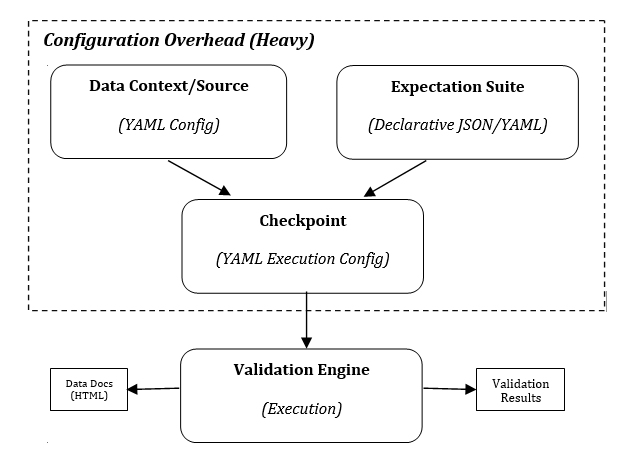
\includegraphics[keepaspectratio]{latex_media/media/image1.png}}

Figure 1: Illustration of the Great Expectations: Configuration vs.
Computation Workflow. While computationally robust, the operational
burden is heavily skewed toward configuration, requiring developers to
orchestrate multiple interconnected YAML and JSON artifacts (Data
Contexts, Expectation Suites, and Checkpoints) before data validation
can execute.

Deepchecks (Deepchecks Inc., 2021) extends profiling to explicit
train/test integrity comparisons, particularly for ML dataset
validation. Its scope is broader but its dependency footprint is
heavier.

Evidently AI (Evidently AI, 2021) focuses specifically on ML monitoring,
providing rich drift detection reports optimized for model monitoring
dashboards. Like YData-Profiling, it excels in exploratory analysis but
is not designed for low-overhead, programmatic integration at the batch
ingestion layer.

The gap in this landscape is a tool that: (a) requires zero
configuration to deploy, (b) returns anomalies as structured Python
objects (not just an HTML report), (c) supports programmatic row-level
extraction, (d) integrates drift detection as a first-class feature, and
(e) maintains a minimal computational footprint at any dataset scale.

\subsubsection{2.2 Statistical Drift
Detection}\label{statistical-drift-detection}

Distribution drift is the phenomenon where the statistical properties of
a dataset change over time. This has been extensively studied in the
context of machine learning monitoring (Widmer \& Kubat, 1996; Gama et
al., 2014). It is typically categorized into two types:

\begin{itemize}
\item
  Covariate Shift (P(X) drift): The distribution of input features
  changes, while the relationship P (Y\textbar X) remains stable.
\item
  Concept Drift (P (Y\textbar X) drift): The relationship between
  features and labels changes, potentially while P(X) remains stable.
\end{itemize}

The Population Stability Index (PSI) was originally developed in the
credit risk industry (Wu \& Bacon, 1999; Siddiqi, 2006) to monitor
shifts in borrower score distributions between model development and
deployment. It has since become a standard metric in MLOps pipelines
(Klaise et al., 2020). The PSI's primary advantage is its
interpretability, as its industry-standard thresholds (\textless{} 0.1:
stable; 0.1--0.25: moderate; ≥ 0.25: significant) provide immediately
actionable severity classifications.

The Kolmogorov-Smirnov (KS) two-sample test (Kolmogorov, 1933; Smirnov,
1948) offers a complementary perspective: while PSI quantifies the
magnitude of distributional shift via information divergence, the KS
test quantifies whether the two samples are statistically consistent
with having been drawn from the same underlying distribution, expressed
as a p-value. Together, PSI and KS provide both quantitative severity
and statistical significance for drift characterization.

\subsubsection{2.3 AI-Augmented Data
Remediation}\label{ai-augmented-data-remediation}

The use of large language models (LLMs) as code-generation engines for
data transformation tasks is an emerging research area. Choi et
al.~(2022) demonstrated that LLMs can generate syntactically correct and
semantically appropriate pandas transformation code when provided with
structured context about a dataset. Recent works, such as the position
paper by Xu et al.~(2024) and comprehensive surveys by Zhou et
al.~(2026), have emphasized the increasingly agentic role of LLMs in
automating data preparation and cleaning workflows. PyDataQuality's AI
Remediation Prompt generator operationalizes this capability by
automatically compiling detected issues, dataset statistics, and column
metadata into a structured prompt template that can be submitted to any
LLM API (ChatGPT, Claude, Gemini) to generate ready-to-execute data
cleaning scripts thereby reducing the remediation cycle from hours of
manual scripting to seconds of AI-assisted automation.

\subsection{III. System Design and
Architecture}\label{iii.-system-design-and-architecture}

\subsubsection{3.1 Design Philosophy}\label{design-philosophy}

PyDataQuality was designed around five explicit architectural principles
that distinguish it from existing tools:

\begin{enumerate}
\def\labelenumi{\arabic{enumi}.}
\item
  Zero-Configuration Deployment: A user should be able to call
  \texttt{pdq.analyze\_dataframe(df)} on any pandas DataFrame without
  configuring schemas, expectation suites, or YAML files. The library
  auto-detects column types and applies appropriate statistical audits.
\item
  Actionable Output Over Descriptive Output: The system produces
  \texttt{QualityIssue} objects with structured severity classifications
  (\texttt{critical}, \texttt{warning}, \texttt{info}) and an explicit
  \texttt{affected\_count} and \texttt{affected\_percentage}. This
  enables programmatic downstream filtering without parsing HTML or
  text.
\item
  Programmatic Row Isolation: The \texttt{get\_problematic\_rows()}
  method returns the actual subset of the DataFrame containing anomalous
  records, enabling downstream deduplication, quarantine, or human
  review workflows.
\item
  Computational Efficiency by Design: The sampling engine decouples
  analysis throughput from dataset size, achieving constant-complexity
  audits regardless of how large the source file is.
\item
  Statistical Rigor Without Heavy Dependencies: Core statistical
  algorithms (IQR, PSI, KS Test) are implemented using only NumPy as the
  computational backend, with optional SciPy acceleration when
  available.
\end{enumerate}

\subsubsection{3.2 System Architecture}\label{system-architecture}

PyDataQuality is organized into five decoupled layers, each with a
single well-defined responsibility:

\begin{longtable}[]{@{}
  >{\raggedright\arraybackslash}p{(\linewidth - 0\tabcolsep) * \real{0.5857}}@{}}
\caption{Figure 2: PyDataQuality Architecture Stack. System architecture
diagram illustrating the 5-layer decoupled design of PyDataQuality. Data
flows from ingestion through an
\pandocbounded{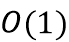
\includegraphics[keepaspectratio]{latex_media/media/image3.png}}-capped
sampling engine, into a core profiling kernel, optionally through a
drift \& decision engine, and finally to the presentation layer for
dashboarding and AI remediation generation.}\tabularnewline
\toprule\noalign{}
\endfirsthead
\endhead
\bottomrule\noalign{}
\endlastfoot
\pandocbounded{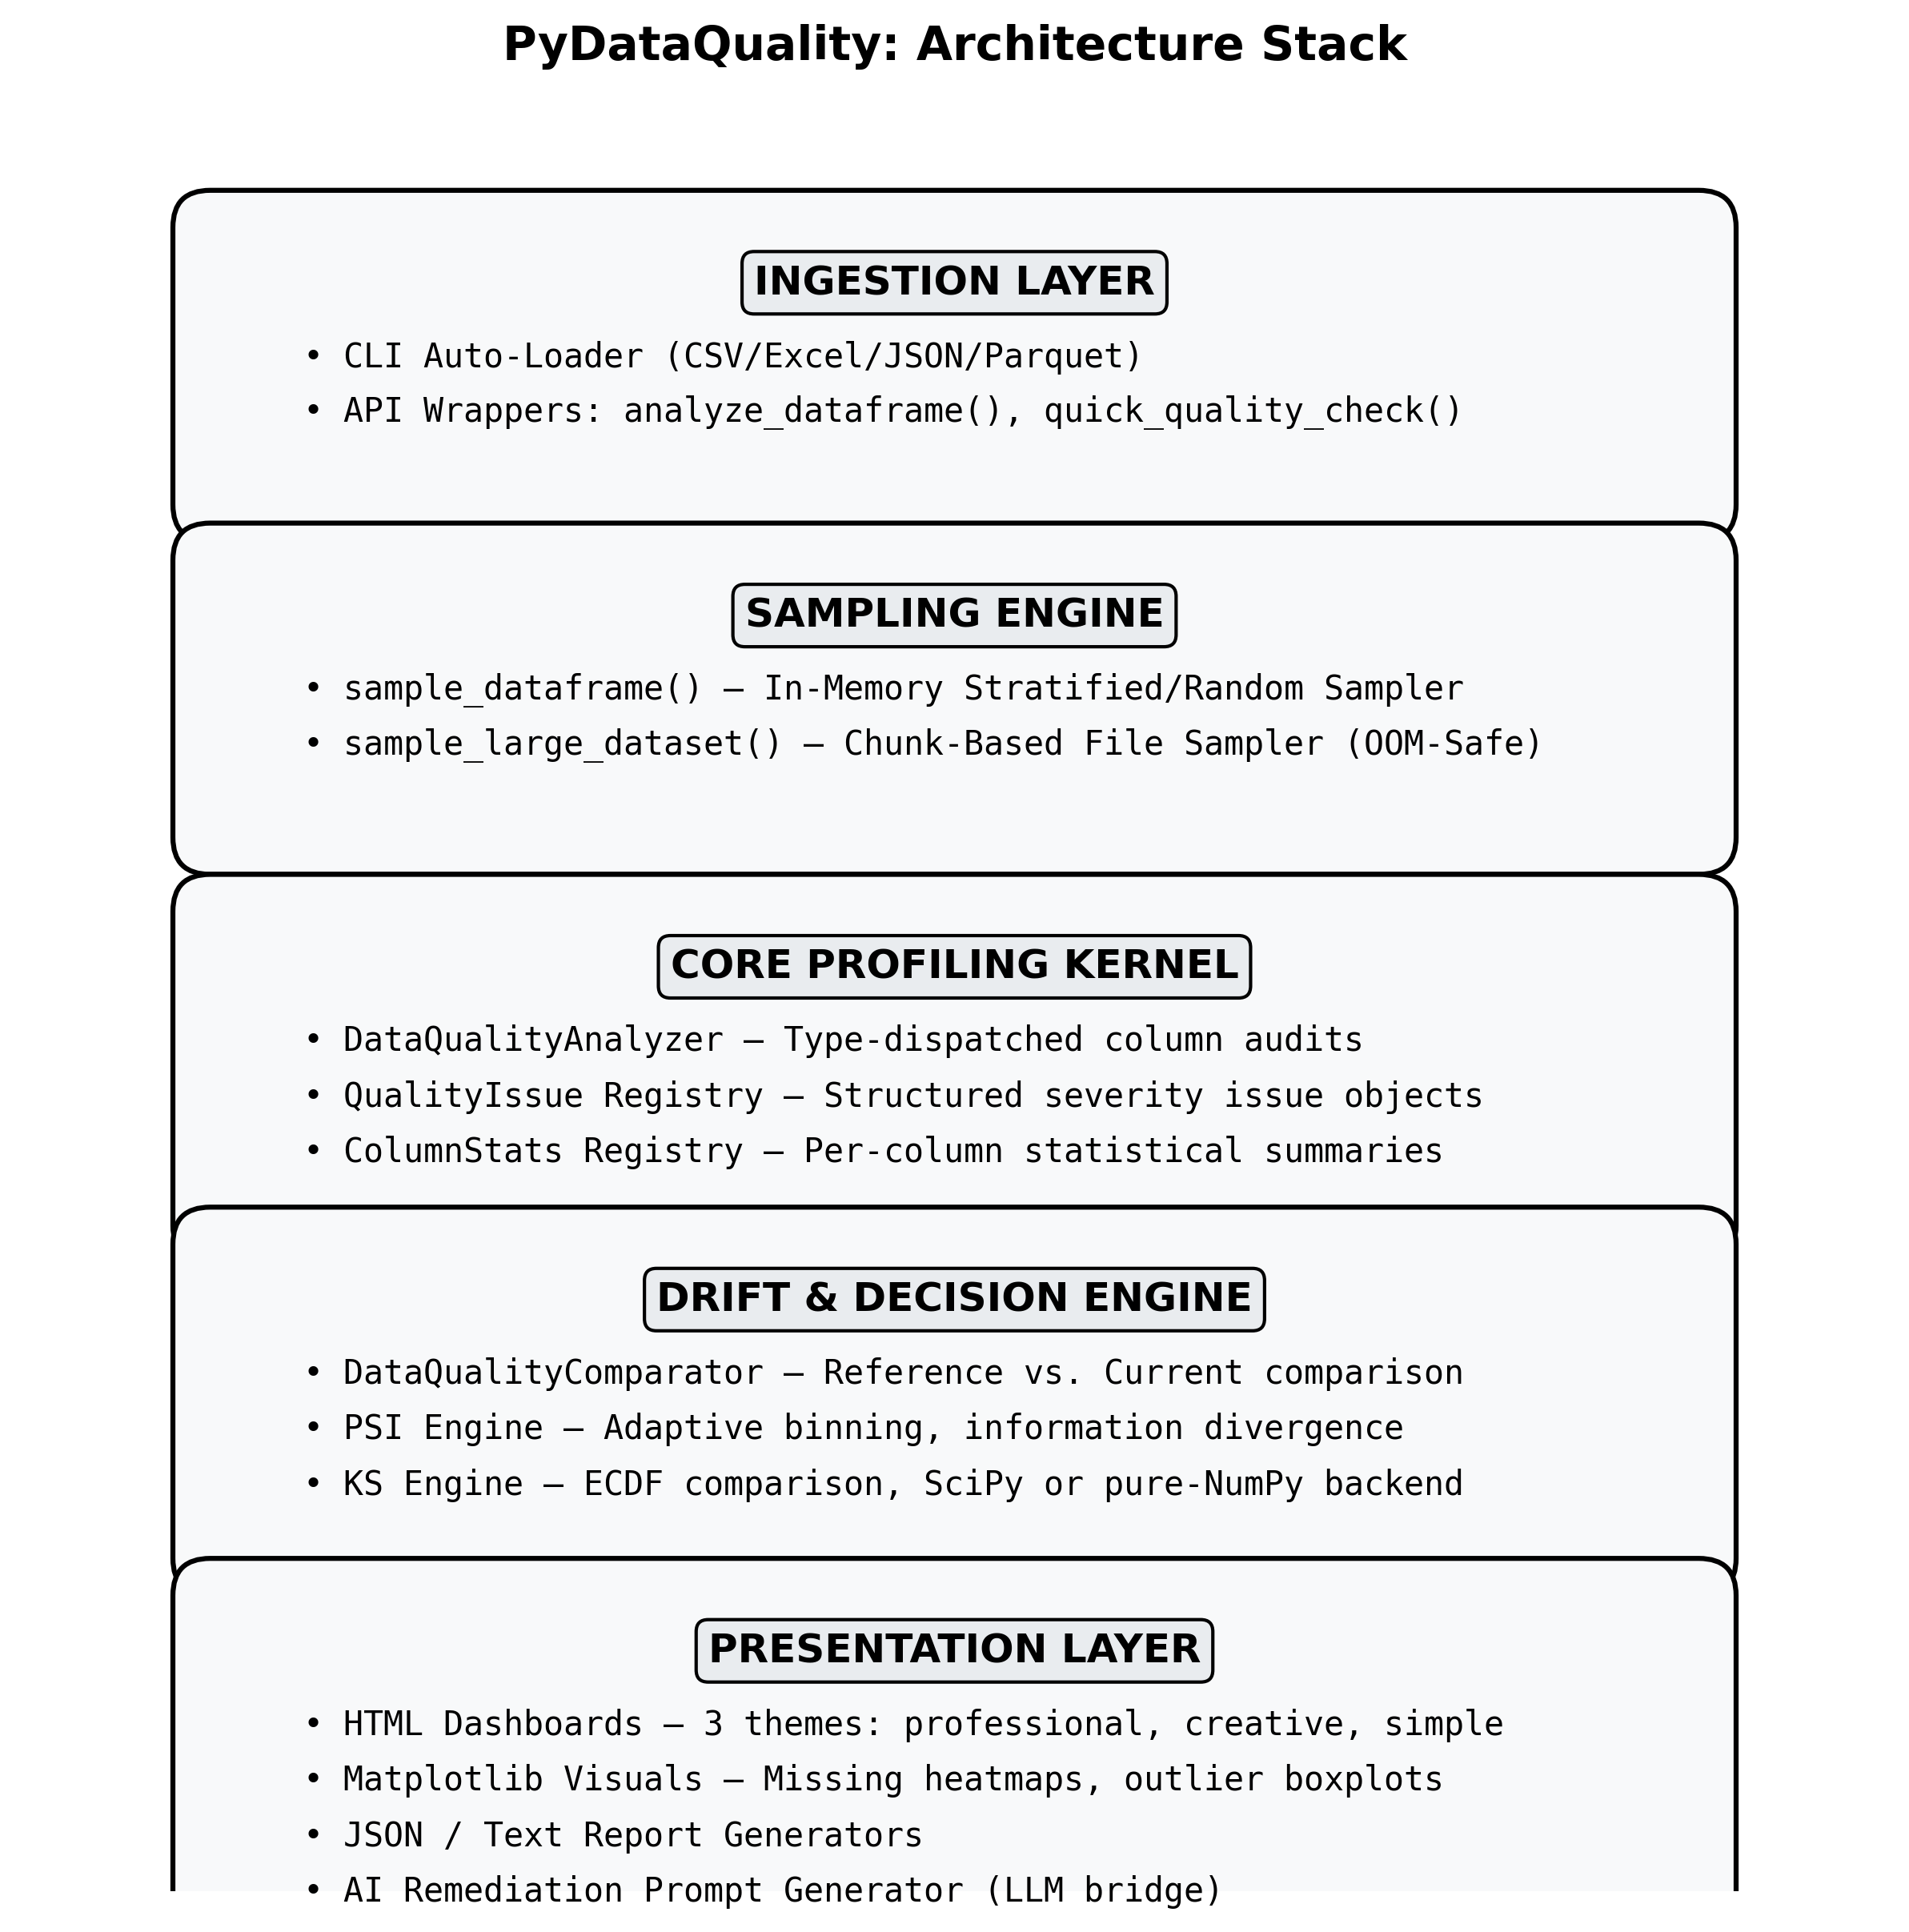
\includegraphics[keepaspectratio]{latex_media/media/image2.png}} \\
\end{longtable}

\subsubsection{3.6.1 Type-Dispatch Visual
Reference}\label{type-dispatch-visual-reference}

Figure 3 provides a visual reference for the analysis matrix, showing
which statistical checks are applied per data type.

\pandocbounded{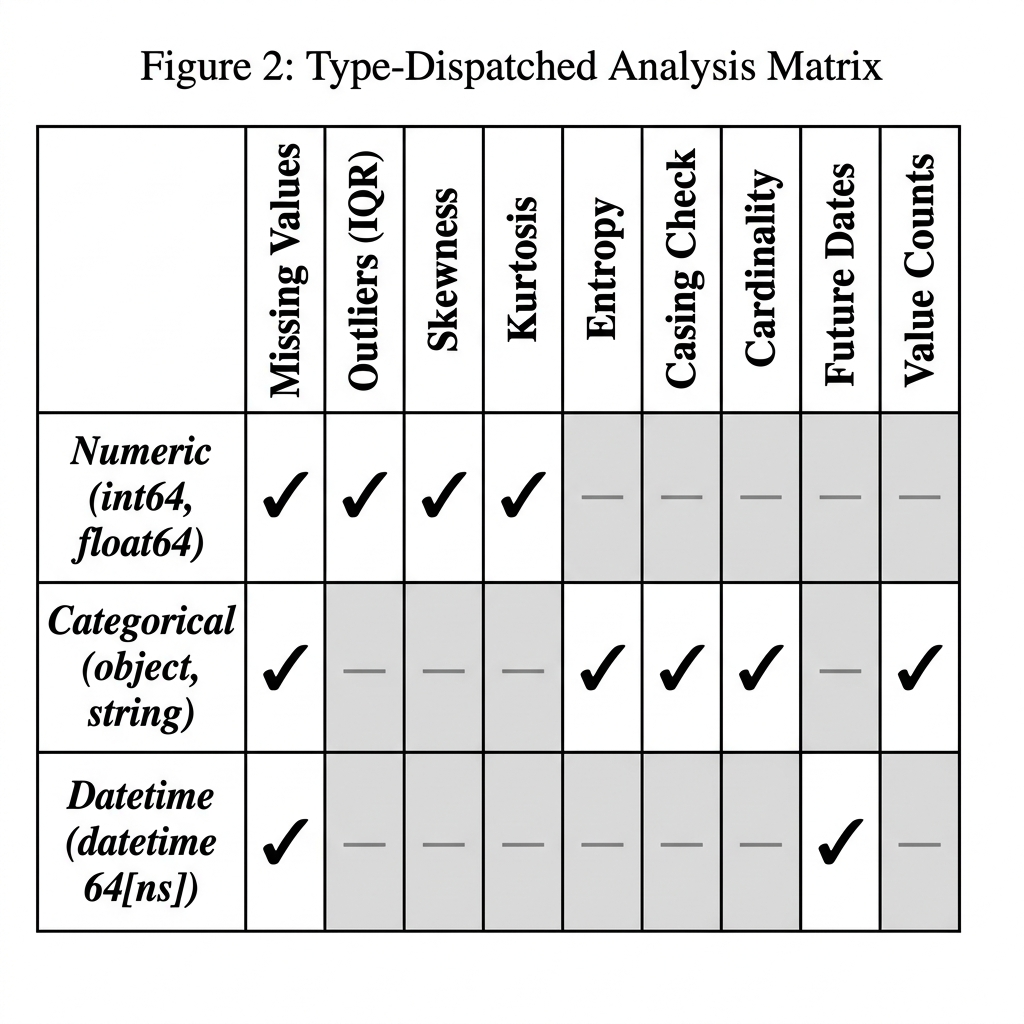
\includegraphics[keepaspectratio]{latex_media/media/image4.jpeg}}

Figure 3: Type-Dispatched Analysis Matrix. Each column type receives a
different set of statistical audits. The checkmarks (✓) indicate the
check is applied; dashes indicate it is not applicable. This dispatch
design prevents, for example, IQR outlier computation being applied to
categorical string columns where it is mathematically undefined.

\subsubsection{3.6.2 Issue Severity
Taxonomy}\label{issue-severity-taxonomy}

Figure 4 illustrates the hierarchical severity classification structure
applied to all detected quality issues.

\pandocbounded{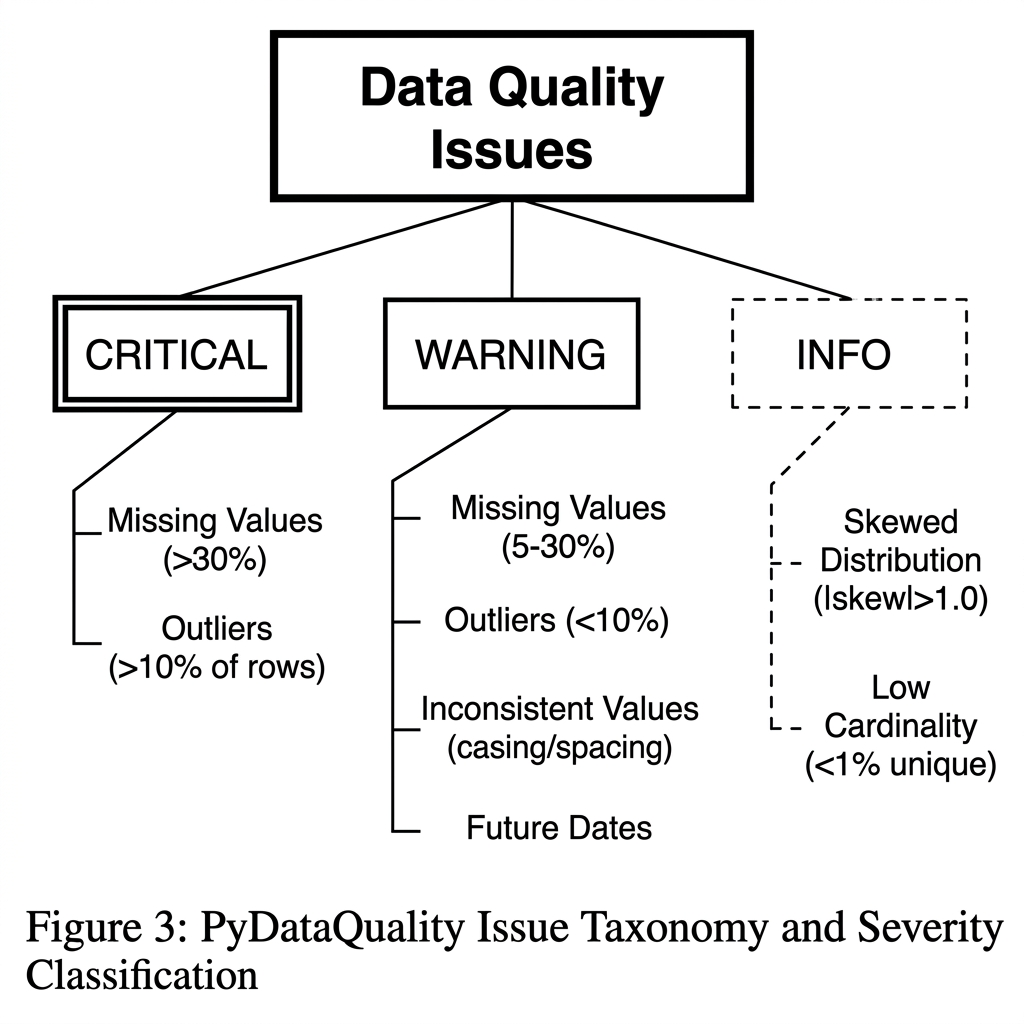
\includegraphics[keepaspectratio]{latex_media/media/image5.jpeg}}

\textbf{Figure 4:} PyDataQuality Issue Taxonomy and Severity
Classification. Issues are stratified into three severity tiers
(CRITICAL, WARNING, and INFO). This enables downstream systems to
respond proportionally. CRITICAL issues (\textgreater30\% missing,
\textgreater10\% outliers) should halt processing; WARNING issues
require investigation; INFO issues are advisory.

\subsubsection{3.3 Layer 1: The Ingestion
Layer}\label{layer-1-the-ingestion-layer}

The ingestion layer provides two entry points:

Python API: The primary interface is
\texttt{pyda}\texttt{taquality.analyze\_dataframe(df,\ name,}\texttt{config)},
which accepts a pandas DataFrame and returns a fully initialized
\texttt{DataQualityAnalyzer} instance. A lighter-weight
\texttt{quick\_quality\_check(df)} function returns only the JSON
summary dictionary for minimal-overhead spot checks.

CLI Interface: The command-line interface accepts any supported file
format and automatically dispatches to the correct pandas reader:

pydataquality -\/-file data.csv -\/-format html -\/-output report.html

pydataquality -\/-file transactions.parquet -\/-format json

The CLI uses \texttt{argparse} for argument parsing and provides clear,
human-readable error messages for unsupported formats or invalid file
paths.

\subsubsection{3.4 Layer 2: The Sampling
Engine}\label{layer-2-the-sampling-engine}

The sampling engine contains two utility functions designed to decouple
analysis cost from data volume:

In-Memory Sampler (\texttt{sample\_dataframe}): For DataFrames already
loaded into memory, this function implements stratified sampling via
\texttt{groupby().apply()} when a \texttt{stratify\_by} column is
specified, ensuring class representation is preserved in the sample. It
falls back to uniform random sampling when stratification fails or is
not requested.

Chunk-Based File Sampler (\texttt{sample\_large\_dataset}): For files
that cannot be loaded entirely into memory, this function reads the file
in configurable chunks (default: 100,000 rows per chunk) using pandas'
\texttt{chunksize} parameter. From each chunk, 10\% of rows are sampled
at random. Chunks are accumulated until the target sample size
multiplied by a coverage factor (5×) is reached, then a final random
down sampling step brings the total to exactly \texttt{n\_samples} rows.
This approach prevents Out-Of-Memory (OOM) failures on files that would
otherwise exhaust available system RAM.

\subsubsection{3.5 Layer 3: The Core Profiling
Kernel}\label{layer-3-the-core-profiling-kernel}

The profiling kernel is implemented in the \texttt{DataQualityAnalyzer}
class, which orchestrates the full analysis lifecycle. Upon
initialization, the analyzer immediately triggers
\texttt{\_analyze\_dataset\_structure()} and then
\texttt{\_analyze\_columns()}, ensuring the analysis is complete by the
time the constructor returns.

\textbf{Type-Dispatching:} The \texttt{\_analyze\_single\_column()}
method inspects each column's dtype using pandas' \texttt{pd.api.types}
introspection functions and dispatches to one of three specialized
analyzers:

\textbf{Table A: Type-Dispatched Analysis Matrix}

{\def\LTcaptype{none} % do not increment counter
\begin{longtable}[]{@{}
  >{\raggedright\arraybackslash}p{(\linewidth - 4\tabcolsep) * \real{0.2662}}
  >{\raggedright\arraybackslash}p{(\linewidth - 4\tabcolsep) * \real{0.3206}}
  >{\raggedright\arraybackslash}p{(\linewidth - 4\tabcolsep) * \real{0.4133}}@{}}
\toprule\noalign{}
\begin{minipage}[b]{\linewidth}\raggedright
pandas dtype family
\end{minipage} & \begin{minipage}[b]{\linewidth}\raggedright
Dispatcher
\end{minipage} & \begin{minipage}[b]{\linewidth}\raggedright
Checks Applied
\end{minipage} \\
\midrule\noalign{}
\endhead
\bottomrule\noalign{}
\endlastfoot
\texttt{int64}, \texttt{float64}, \texttt{bool} &
\texttt{\_analyze\_numeric\_column} & Mean, std, min, max, median, Q1,
Q3, skewness, kurtosis, zero count, IQR outliers \\
\texttt{object}, \texttt{string}, \texttt{category} &
\texttt{\_analyze\_categorical\_column} & Value counts, mode, mode
frequency, Shannon entropy, casing/spacing inconsistencies \\
\texttt{datetime64{[}ns{]}} & \texttt{\_analyze\_datetime\_column} &
Date range, future date count, min/max timestamps \\
\end{longtable}
}

\textbf{The} \texttt{QualityIssue} \textbf{Dataclass:} Each detected
anomaly is encapsulated as a \texttt{QualityIssue} instance with the
following fields:

@dataclass

class QualityIssue:

column: str \# Column name where the issue was detected

issue\_type: str \# e.g.
\textquotesingle missing\_values\textquotesingle,
\textquotesingle outliers\textquotesingle,
\textquotesingle inconsistent\_values\textquotesingle{}

severity: str \# \textquotesingle critical\textquotesingle,
\textquotesingle warning\textquotesingle, or
\textquotesingle info\textquotesingle{}

message: str \# Human-readable explanation with numerical details

affected\_count: int \# Number of rows affected

affected\_percentage: float \# Percentage of total rows affected

details: Dict \# Extended metadata (bounds, examples, thresholds)

This structured representation enables downstream code to
programmatically filter issues by severity
(\texttt{{[}i~for~i~in~analyzer.issues~if~i.severity~==~critical}),
aggregate by type, or serialize to JSON for integration with monitoring
dashboards.

\textbf{Configurable Thresholds:} The profiling kernel is governed by a
configuration dictionary (\texttt{QUALITY\_THRESHOLDS}) that exposes all
detection thresholds as tunable parameters:

QUALITY\_THRESHOLDS = \{

"missing\_critical": 0.30, \# \textgreater30\% missing = critical

"missing\_warning": 0.05, \# \textgreater5\% missing = warning

"outlier\_threshold": 1.5, \# IQR multiplier (k)

"skew\_threshold": 1.0, \# \textbar skewness\textbar{} \textgreater{}
1.0 = skewed

"unique\_threshold": 0.01, \# uniqueness ratio \textless{} 1\% = low
cardinality

"zero\_threshold": 0.80, \# \textgreater80\% zeros = suspicious

A user can override any of these by passing a \texttt{config} dictionary
to \texttt{analyze\_dataframe()}:

\emph{\# Example: tighten outlier detection and lower missing threshold}

\emph{strict\_analyzer = pdq.analyze\_dataframe(df, config=\{}

\emph{"outlier\_threshold": 3.0, \# Tukey standard: k=3.0 for extreme
outliers}

\emph{"missing\_warning": 0.01 \# Flag even 1\% missing as a warning}

\emph{\})}

\textbf{The} \texttt{get\_problematic\_rows()} \textbf{Method:} This is
arguably the most operationally valuable method in PyDataQuality. Rather
than simply \emph{reporting} that a column has outliers, this method
returns the actual problematic rows as a new DataFrame:

\emph{\# Get all rows where age is an outlier} outlier\_rows =
analyzer.get\_problematic\_rows(age, issue\_type=outliers)

\emph{\# Get all rows with missing income} missing\_income =
analyzer.get\_problematic\_rows(income, issue\_type=missing\_values)

\emph{\# Get union of all issues in a column} all\_age\_problems =
analyzer.get\_problematic\_rows(age, issue\_type=all)

The method constructs a boolean mask using the same IQR boundaries
computed during the analysis phase, ensuring consistency between
reported issue counts and the returned subset. This enables workflows
such as:

\begin{itemize}
\item
  Data Quarantine: Routing anomalous rows to a separate storage table
  for human review
\item
  Audit Logging: Preserving a record of exactly which rows were flagged
  and why before cleaning
\item
  Differential Analysis: Comparing the statistical properties of
  problematic vs.~clean subsets
\end{itemize}

\textbf{Empirical Validation of}
\texttt{get\_problematic\_rows()}\textbf{:} In our verification
experiment, we constructed a 12-row dataset with two known age outliers
(-100 and 999) and two missing income values. The
\texttt{get\_problematic\_rows()} method correctly isolated exactly the
two outlier rows:

\texttt{Age\ outlier\ rows\ detected:\ 2\ (out\ of\ 12)}

\texttt{Row\ 3:\ \ age\ =\ -100,\ }\texttt{income\ =\ 48000.0}

\texttt{Row\ 5:\ \ age\ =\ 999,}\texttt{\ }\texttt{\ income\ =\ 51000.0}

The two missing income rows were correctly recovered via
\texttt{get\_problematic\_}\texttt{rows\ (}\texttt{income,~missing\_values)},
and the union-mode \texttt{all} returned exactly 2 rows for the age
column (only outlier flags, as there were no missing age values). This
confirms the mask logic is implemented correctly and consistently.

\subsubsection{3.6 Layer 4: The Drift and Decision
Engine}\label{layer-4-the-drift-and-decision-engine}

The drift engine is implemented in \texttt{DataQualityComparator}, which
accepts two \texttt{DataQualityAnalyzer} instances (reference and
current) and computes distributional comparison metrics for all shared
columns.

\emph{\# Typical usage in a production pipeline}

\emph{train\_analyzer = pdq.analyze\_dataframe(df\_train, name="Training
Baseline")}

\emph{prod\_analyzer = pdq.analyze\_dataframe(df\_live, name="Live
Production")}

\emph{drift\_report = pdq.compare\_drift(train\_analyzer,
prod\_analyzer)}

The \texttt{compare\_drift()} convenience function returns a pandas
DataFrame where each row represents one column and columns include:
\texttt{column}, \texttt{dtype}, \texttt{psi}, \texttt{drift\_status},
\texttt{pct\_change}, \texttt{ks\_statistic}, \texttt{ks\_p\_value}.

\subsubsection{3.7 Layer 5: The Presentation
Layer}\label{layer-5-the-presentation-layer}

The presentation layer offers multiple output modalities:

\textbf{HTML Dashboard Themes:}

\texttt{professional}: Clean white background, optimized for PDF export
and formal reporting

\texttt{creative}: Dark-mode gradient design with animated cards,
optimized for interactive web presentation

\texttt{simple}: Minimal HTML with inline styles for maximum
compatibility

\textbf{Matplotlib Visualizations:} The \texttt{DataQualityVisualizer}
class generates:

Missing data heatmaps (showing null patterns as a 2D matrix)

Outlier distribution boxplots

Correlation heatmaps using the \texttt{coolwarm} colormap

Issue severity distribution pie charts and bar charts

\textbf{AI Remediation Prompt Generator:} Described in detail in Section
III.8.

\subsubsection{3.8 The AI Remediation Prompt
Generator}\label{the-ai-remediation-prompt-generator}

A unique capability of PyDataQuality is its
\texttt{generate\_ai\_prompt()} function, which dynamically compiles a
structured remediation prompt from the detected issues and dataset
statistics:

prompt = pdq.generate\_ai\_prompt(analyzer)

print(prompt)

\# Copy to ChatGPT / Claude / Gemini → receive ready-to-run cleaning
script

The generated prompt includes: 1. A dataset summary (shape, memory
usage, column types) 2. A structured list of all detected quality issues
with severities and affected counts 3. Key statistical statistics per
column (mean, std, missing \%, outlier bounds) 4. A request
specification asking the AI to generate executable Python/pandas code to
address each issue systematically

This feature bridges static analysis with generative AI, reducing the
time from ``data quality issue detected'' to ``cleaning code generated
and ready to execute'' from hours of manual scripting to seconds of
AI-assisted automation.

\subsection{IV. Mathematical Formulations and Statistical
Engine}\label{iv.-mathematical-formulations-and-statistical-engine}

This section provides complete mathematical derivations of all four
statistical algorithms implemented in PyDataQuality, with concrete
numerical worked examples verified against our experimental outputs.

\subsubsection{4.1 Shannon Entropy for Categorical
Uniformity}\label{shannon-entropy-for-categorical-uniformity}

\pandocbounded{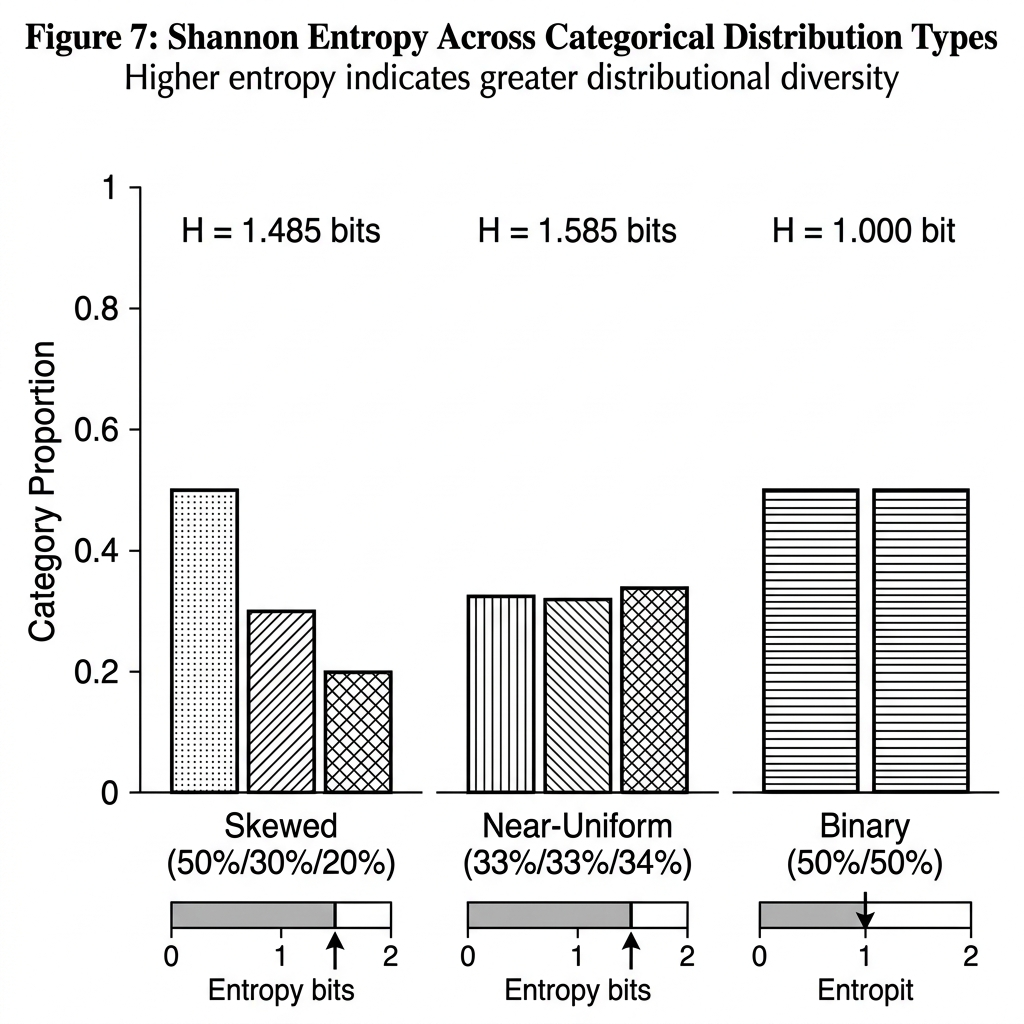
\includegraphics[keepaspectratio]{latex_media/media/image6.jpeg}}

\textbf{Figure 5:} Shannon Entropy comparison across three
representative categorical distributions. Skewed distributions
(50/30/20) yield lower entropy (1.485 bits) indicating dominant class
imbalance. Near-uniform distributions approach the theoretical maximum
of
\pandocbounded{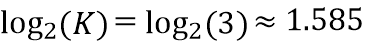
\includegraphics[keepaspectratio]{latex_media/media/image7.png}}
bits. Binary balanced distributions produce exactly 1.000 bit, the
fundamental unit of binary information. PyDataQuality reports entropy as
a column statistic, enabling detection of degenerate features (entropy ≈
0) indicating near-constant columns.

For categorical columns, PyDataQuality computes Shannon Entropy
(Shannon, 1948) to measure the distributional diversity of a categorical
feature. A low-entropy column (e.g., 99\% of values are ``A'') may
indicate domain leakage, label imbalance, or degenerate data; a
high-entropy column indicates healthy diversity.

\textbf{Definition:} Given a categorical feature vector
\pandocbounded{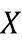
\includegraphics[keepaspectratio]{latex_media/media/image8.png}}
with
\pandocbounded{
\includegraphics[keepaspectratio]{latex_media/media/image9.png}}
distinct categories
\pandocbounded{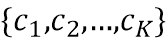
\includegraphics[keepaspectratio]{latex_media/media/image10.png}},
and the empirical probability of each category:

\pandocbounded{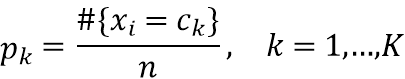
\includegraphics[keepaspectratio]{latex_media/media/image11.png}}

The \textbf{Shannon Entropy}
\pandocbounded{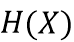
\includegraphics[keepaspectratio]{latex_media/media/image12.png}}
is defined as:

\pandocbounded{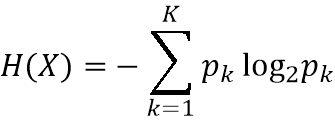
\includegraphics[keepaspectratio]{latex_media/media/image13.png}}

Where entropy is measured in bits. The maximum possible entropy for
\pandocbounded{
\includegraphics[keepaspectratio]{latex_media/media/image9.png}}
classes is
\pandocbounded{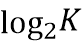
\includegraphics[keepaspectratio]{latex_media/media/image14.png}}
bits (achieved when all classes are equally probable, i.e.,
\pandocbounded{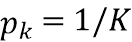
\includegraphics[keepaspectratio]{latex_media/media/image15.png}}
for all
\pandocbounded{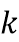
\includegraphics[keepaspectratio]{latex_media/media/image16.png}}),
and the minimum is 0 bits (achieved when all observations belong to a
single class).

\textbf{Worked Numerical Example (verified empirically):}

\emph{Experiment 1: Skewed distribution (50/30/20 split across 3
categories)}

\pandocbounded{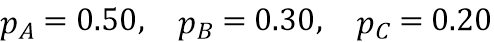
\includegraphics[keepaspectratio]{latex_media/media/image17.png}}

\pandocbounded{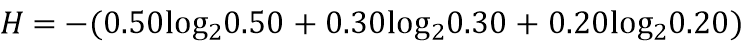
\includegraphics[keepaspectratio]{latex_media/media/image18.png}}

\pandocbounded{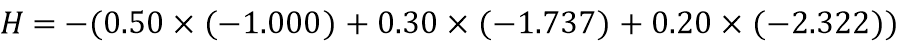
\includegraphics[keepaspectratio]{latex_media/media/image19.png}}

\pandocbounded{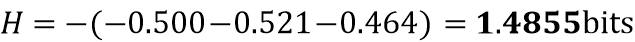
\includegraphics[keepaspectratio]{latex_media/media/image20.png}}

\emph{Our system output:} \texttt{1.485475~bits}

\emph{Experiment 2: Near-uniform distribution (33/33/34 split)}

\pandocbounded{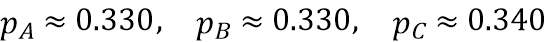
\includegraphics[keepaspectratio]{latex_media/media/image21.png}}

\pandocbounded{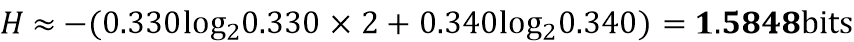
\includegraphics[keepaspectratio]{latex_media/media/image22.png}}

\emph{Our system output:} \texttt{1.584819~bits}

(Note: 1.5848 ≈
\pandocbounded{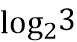
\includegraphics[keepaspectratio]{latex_media/media/image23.png}},
confirming near-maximum entropy)

\emph{Experiment 3: Binary balance (50/50 split)}

\pandocbounded{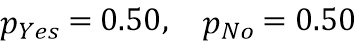
\includegraphics[keepaspectratio]{latex_media/media/image24.png}}

\pandocbounded{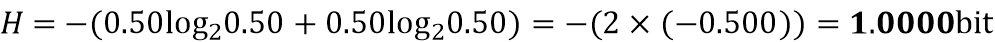
\includegraphics[keepaspectratio]{latex_media/media/image25.png}}

\emph{Our system output:} \texttt{1.000000~bits}

These results confirm the exact mathematical correctness of the entropy
implementation. The results also provide an interpretive benchmark: a
perfectly balanced binary categorical feature (50/50) has exactly 1.0
bit of entropy, 1 bit being the unit of binary information. Any
deviation from 1.0 indicates imbalance; any value approaching
\pandocbounded{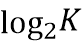
\includegraphics[keepaspectratio]{latex_media/media/image14.png}}
confirms category uniformity.

\subsubsection{4.2 Interquartile Range (IQR) Outlier
Detection}\label{interquartile-range-iqr-outlier-detection}

For continuous numerical features, PyDataQuality implements the
\textbf{Tukey Fence} method (Tukey, 1977), the gold standard for
non-parametric outlier detection that makes no assumption about the
underlying distribution's normality.

\textbf{Algorithm:} Given a numerical feature vector
\pandocbounded{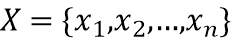
\includegraphics[keepaspectratio]{latex_media/media/image26.png}}
(after removing missing values):

\textbf{Step 1: Compute Quartiles:}

\pandocbounded{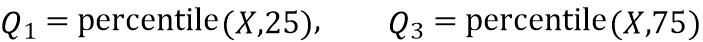
\includegraphics[keepaspectratio]{latex_media/media/image27.png}}

\textbf{Step 2: Compute Interquartile Range:}

\pandocbounded{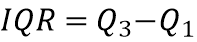
\includegraphics[keepaspectratio]{latex_media/media/image28.png}}

\textbf{Step 3: Establish Validation Fences} (using configurable
multiplier
\pandocbounded{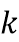
\includegraphics[keepaspectratio]{latex_media/media/image16.png}},
default
\pandocbounded{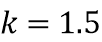
\includegraphics[keepaspectratio]{latex_media/media/image29.png}}):

\pandocbounded{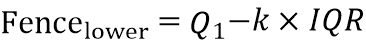
\includegraphics[keepaspectratio]{latex_media/media/image30.png}}

\pandocbounded{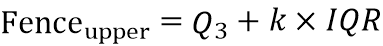
\includegraphics[keepaspectratio]{latex_media/media/image31.png}}

\textbf{Step 4: Flag Outliers:} Any sample
\pandocbounded{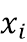
\includegraphics[keepaspectratio]{latex_media/media/image32.png}}
satisfying:

\pandocbounded{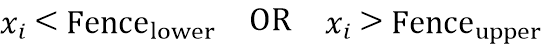
\includegraphics[keepaspectratio]{latex_media/media/image33.png}}

is registered as a \texttt{QualityIssue} with
\texttt{issue\_type="outliers"}.

\textbf{Severity Escalation:} An outlier issue is classified as:

\begin{itemize}
\item
  \texttt{severity="warning"} if the outlier percentage is \textless{}
  10\% of the total non-null sample
\item
  \texttt{severity="critical"} if the outlier percentage is ≥ 10\% of
  the total non-null sample
\end{itemize}

The configurable multiplier
\pandocbounded{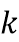
\includegraphics[keepaspectratio]{latex_media/media/image16.png}}
allows users to choose between two standard regimes:

\begin{itemize}
\item
  \pandocbounded{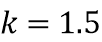
\includegraphics[keepaspectratio]{latex_media/media/image29.png}}:
  \textbf{Standard Tukey fences} flags \emph{mild} outliers; appropriate
  for most general-purpose quality audits
\item
  \pandocbounded{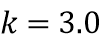
\includegraphics[keepaspectratio]{latex_media/media/image34.png}}:
  \textbf{Extreme outlier fences} flags only severe outliers;
  appropriate for domains (e.g., sensor data) where significant natural
  variance is expected
\end{itemize}

\textbf{Worked Numerical Example (verified empirically):}

Dataset:
\pandocbounded{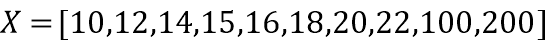
\includegraphics[keepaspectratio]{latex_media/media/image35.png}}

Step 1:
\pandocbounded{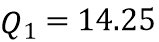
\includegraphics[keepaspectratio]{latex_media/media/image36.png}},
\pandocbounded{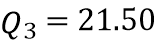
\includegraphics[keepaspectratio]{latex_media/media/image37.png}}

(from \texttt{data.quantile(0.25)} and \texttt{data.quantile(0.75)})

Step 2:
\pandocbounded{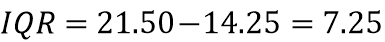
\includegraphics[keepaspectratio]{latex_media/media/image38.png}}

Step 3 (k=1.5):

\pandocbounded{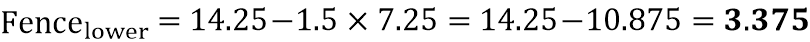
\includegraphics[keepaspectratio]{latex_media/media/image39.png}}

\pandocbounded{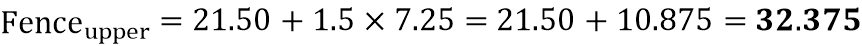
\includegraphics[keepaspectratio]{latex_media/media/image40.png}}

Step 4: Values
\pandocbounded{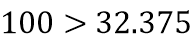
\includegraphics[keepaspectratio]{latex_media/media/image41.png}}
and
\pandocbounded{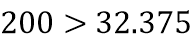
\includegraphics[keepaspectratio]{latex_media/media/image42.png}},
therefore:

\emph{Outliers detected: {[}100, 200{]}}, 2 out of 10 values (20\%)

\emph{Our system output:} \texttt{Outliers:~{[}100,~200{]}}

\pandocbounded{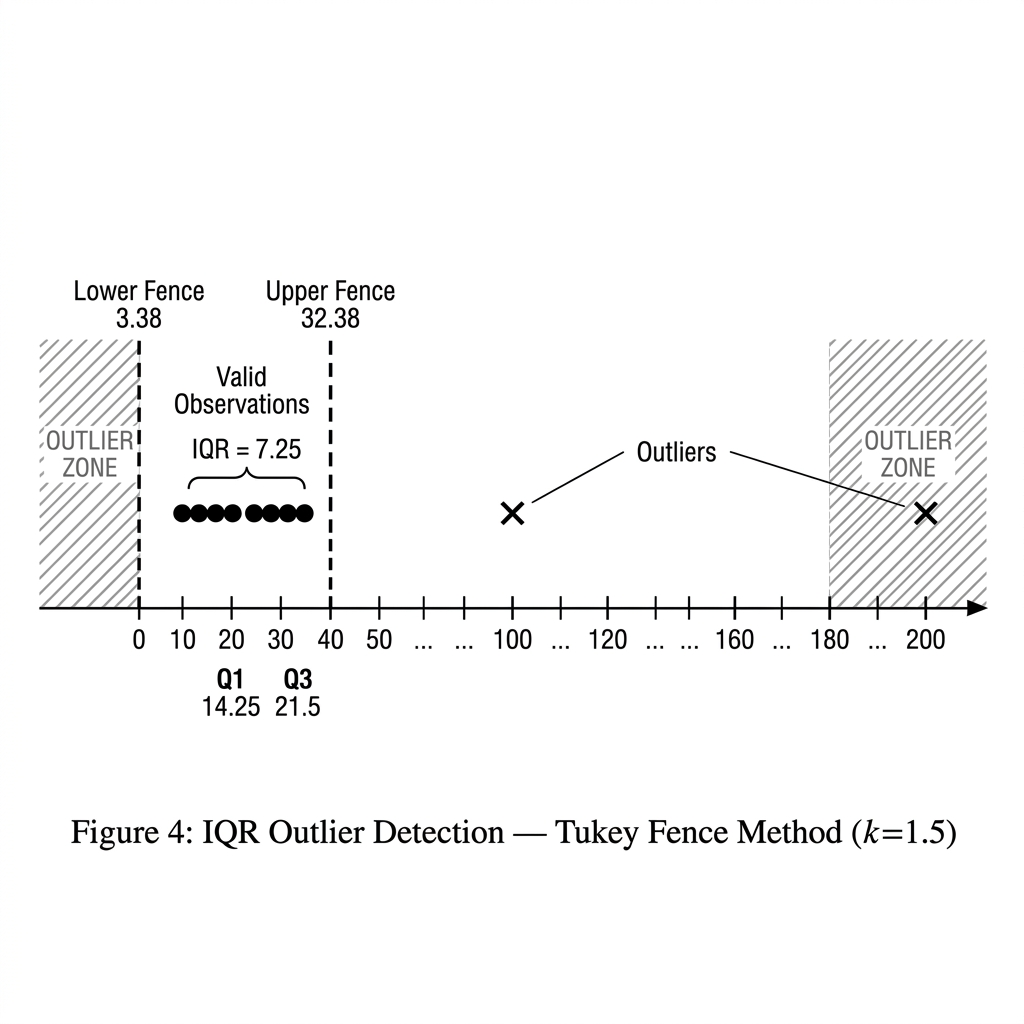
\includegraphics[keepaspectratio]{latex_media/media/image43.jpeg}}

Figure 6: Visual representation of the IQR outlier detection algorithm
on the worked example dataset
\pandocbounded{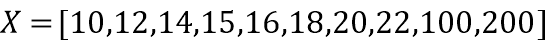
\includegraphics[keepaspectratio]{latex_media/media/image35.png}}.
Blue points lie within the Tukey fences {[}3.38, 32.38{]} and are
classified as valid observations. Red markers at 100 and 200 exceed the
upper fence and are flagged as outliers. The fence is derived from
Q1=14.25, Q3=21.5, IQR=7.25,
\pandocbounded{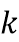
\includegraphics[keepaspectratio]{latex_media/media/image16.png}}=1.5.

\textbf{Why IQR Over Z-Score?} The IQR method is preferred over the
standard Z-score method
(\pandocbounded{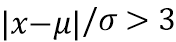
\includegraphics[keepaspectratio]{latex_media/media/image44.png}})
because:

1. The IQR is resistant to the outliers themselves influencing the
detection threshold (Z-score's mean and std are corrupted by extreme
values)

2. The IQR requires no normality assumption, making it appropriate for
skewed financial, income, or sensor distributions

3. Tukey's original formulation (1977) remains the industry standard in
exploratory data analysis precisely for these properties

\subsubsection{4.3 Population Stability Index
(PSI)}\label{population-stability-index-psi}

The Population Stability Index (PSI) was developed in the credit risk
modeling industry (Wu \& Bacon, 1999) to quantify the degree to which a
population's score distribution has shifted between a reference period
(e.g., model training) and a current period (e.g., live deployment). It
has since become a universal metric in MLOps for measuring
distributional drift across any feature type.

\textbf{Mathematical Definition:}

Let
\pandocbounded{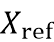
\includegraphics[keepaspectratio]{latex_media/media/image45.png}}
and
\pandocbounded{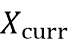
\includegraphics[keepaspectratio]{latex_media/media/image46.png}}
denote the reference and current distributions respectively.

\textbf{For Numerical Columns (Adaptive Decile Binning):}

The reference distribution is used to establish
\pandocbounded{
\includegraphics[keepaspectratio]{latex_media/media/image47.png}}
bins via decile percentiles
(\pandocbounded{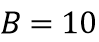
\includegraphics[keepaspectratio]{latex_media/media/image48.png}}
by default):

\pandocbounded{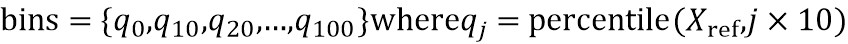
\includegraphics[keepaspectratio]{latex_media/media/image49.png}}

The expected proportion in bin
\pandocbounded{
\includegraphics[keepaspectratio]{latex_media/media/image50.png}}
(from the reference distribution) and actual proportion in bin
\pandocbounded{
\includegraphics[keepaspectratio]{latex_media/media/image50.png}}
(from the current distribution) are:

\pandocbounded{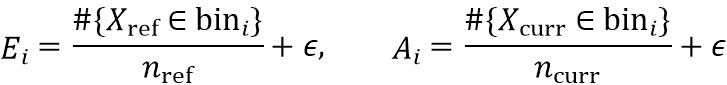
\includegraphics[keepaspectratio]{latex_media/media/image51.png}}

where
\pandocbounded{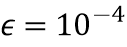
\includegraphics[keepaspectratio]{latex_media/media/image52.png}}
is a regularization constant to prevent division-by-zero or
\pandocbounded{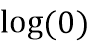
\includegraphics[keepaspectratio]{latex_media/media/image53.png}}
in the KL divergence calculation.

\textbf{For Categorical Columns (Category-Level Binning):}

Each unique category defines its own bin. For a category
\pandocbounded{
\includegraphics[keepaspectratio]{latex_media/media/image54.png}}
in the union of both category sets:

\pandocbounded{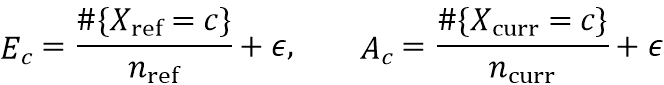
\includegraphics[keepaspectratio]{latex_media/media/image55.png}}

\textbf{PSI Formula} (summed over all bins
\pandocbounded{
\includegraphics[keepaspectratio]{latex_media/media/image47.png}}):

\pandocbounded{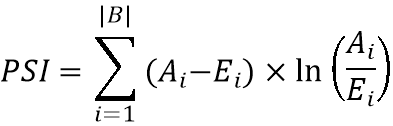
\includegraphics[keepaspectratio]{latex_media/media/image56.png}}

This is equivalent to the symmetric Kullback-Leibler divergence (or
Jensen-Shannon divergence scaled by a factor), measuring the total
information loss from approximating the current distribution with the
reference distribution and vice versa.

\textbf{Drift Severity Classification:}

\textbf{Table B: PSI Drift Severity Classification Thresholds}

{\def\LTcaptype{none} % do not increment counter
\begin{longtable}[]{@{}
  >{\raggedright\arraybackslash}p{(\linewidth - 4\tabcolsep) * \real{0.2236}}
  >{\raggedright\arraybackslash}p{(\linewidth - 4\tabcolsep) * \real{0.2057}}
  >{\raggedright\arraybackslash}p{(\linewidth - 4\tabcolsep) * \real{0.4831}}@{}}
\toprule\noalign{}
\begin{minipage}[b]{\linewidth}\raggedright
PSI Value
\end{minipage} & \begin{minipage}[b]{\linewidth}\raggedright
Classification
\end{minipage} & \begin{minipage}[b]{\linewidth}\raggedright
Recommended Action
\end{minipage} \\
\midrule\noalign{}
\endhead
\bottomrule\noalign{}
\endlastfoot
PSI \textless{} 0.10 & Stable & No action required \\
0.10 ≤ PSI \textless{} 0.25 & Moderate Drift & Investigate root cause;
monitor closely \\
PSI ≥ 0.25 & Significant Drift & Halt inference; trigger model
retraining \\
\end{longtable}
}

\pandocbounded{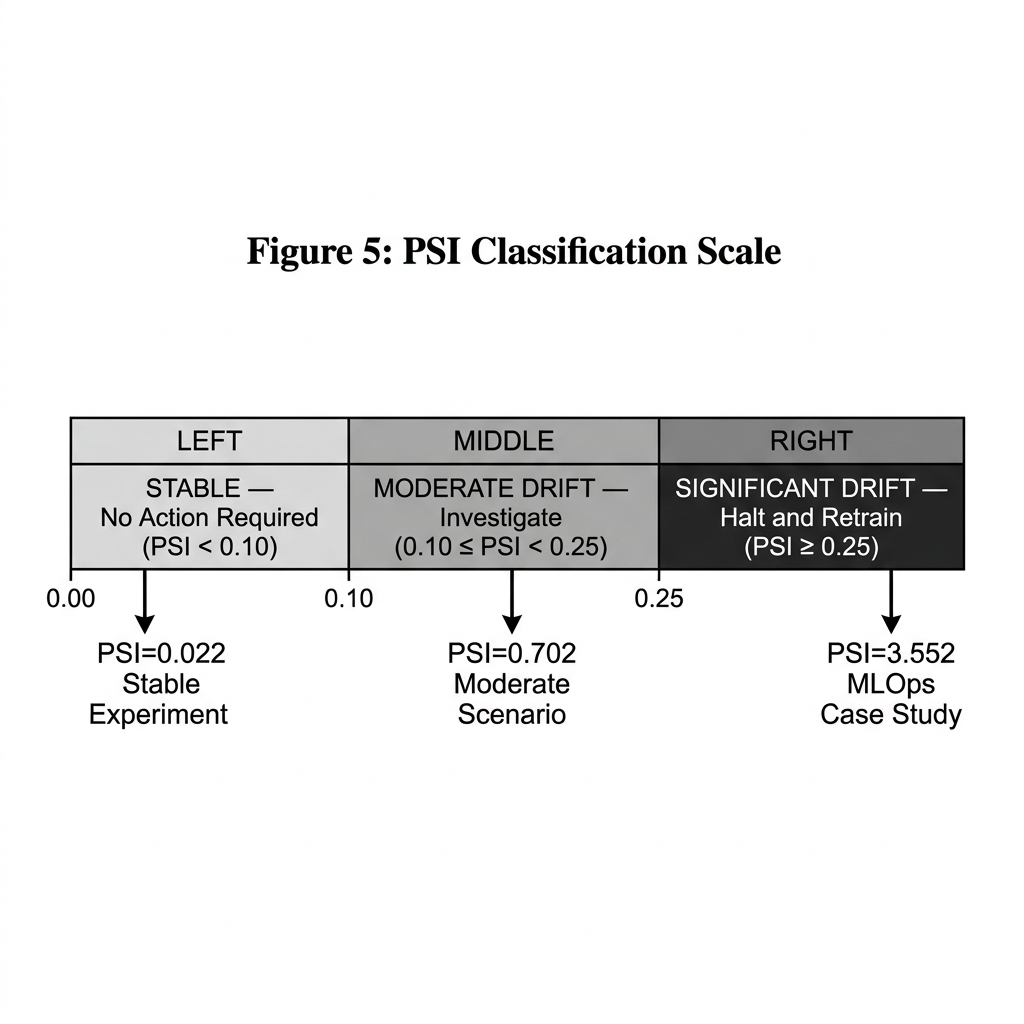
\includegraphics[keepaspectratio]{latex_media/media/image57.jpeg}}

Figure 7: Population Stability Index (PSI) drift severity classification
scale.

The three zones correspond to the industry-standard thresholds derived
from credit risk modeling practice (Wu \& Bacon, 1999). Experimental
values from our verification study are marked: PSI=0.022 (stable
scenario), PSI=0.702 (moderate shift scenario), and PSI=3.552 (MLOps
case study, credit score drift). Note that the PSI scale is unbounded
above; severe drift can produce values far exceeding 1.0.

\textbf{Worked Numerical Example (verified empirically):}

We constructed three controlled scenarios using the same reference
population
(\pandocbounded{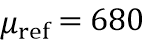
\includegraphics[keepaspectratio]{latex_media/media/image58.png}},
\pandocbounded{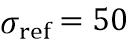
\includegraphics[keepaspectratio]{latex_media/media/image59.png}},
\pandocbounded{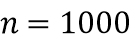
\includegraphics[keepaspectratio]{latex_media/media/image60.png}}):

\textbf{Table C: PSI Verification Results Across Controlled Drift
Scenarios}

{\def\LTcaptype{none} % do not increment counter
\begin{longtable}[]{@{}
  >{\raggedright\arraybackslash}p{(\linewidth - 10\tabcolsep) * \real{0.1323}}
  >{\raggedright\arraybackslash}p{(\linewidth - 10\tabcolsep) * \real{0.1791}}
  >{\raggedright\arraybackslash}p{(\linewidth - 10\tabcolsep) * \real{0.1432}}
  >{\raggedright\arraybackslash}p{(\linewidth - 10\tabcolsep) * \real{0.1824}}
  >{\raggedright\arraybackslash}p{(\linewidth - 10\tabcolsep) * \real{0.1732}}
  >{\raggedright\arraybackslash}p{(\linewidth - 10\tabcolsep) * \real{0.1897}}@{}}
\toprule\noalign{}
\begin{minipage}[b]{\linewidth}\raggedright
Scenario
\end{minipage} & \begin{minipage}[b]{\linewidth}\raggedright
Current Mean
\end{minipage} & \begin{minipage}[b]{\linewidth}\raggedright
Mean Shift
\end{minipage} & \begin{minipage}[b]{\linewidth}\raggedright
Computed PSI
\end{minipage} & \begin{minipage}[b]{\linewidth}\raggedright
Classification
\end{minipage} & \begin{minipage}[b]{\linewidth}\raggedright
System Output
\end{minipage} \\
\midrule\noalign{}
\endhead
\bottomrule\noalign{}
\endlastfoot
Stable & μ = 682 & \textasciitilde2 pts & \textbf{0.0215} & Stable &
\texttt{0.021496} \\
Moderate & μ = 620 & \textasciitilde60 pts & \textbf{0.7020} &
Significant & \texttt{0.702023} \\
Severe & μ = 560 & \textasciitilde120 pts & \textbf{4.6056} &
Significant & \texttt{4.605624} \\
\end{longtable}
}

Note: In the moderate-drift scenario, a 60-point mean shift in a
population with σ=50 (i.e., a 1.2σ shift) is classified as
``significant'' (PSI=0.702). This confirms that PSI is a sensitive
metric, a full standard deviation of distributional shift triggers the
highest alert category, which is the appropriate response in
risk-sensitive applications.

The Severe scenario (120-point shift, 2.4σ) yields PSI = 4.606, which is
orders of magnitude above the 0.25 threshold, confirming that the metric
is not bounded above and can detect catastrophic shifts with
proportionally large values.

\subsubsection{4.4 Two-Sample Kolmogorov-Smirnov
Test}\label{two-sample-kolmogorov-smirnov-test}

The two-sample Kolmogorov-Smirnov (KS) Test (Kolmogorov, 1933; Smirnov,
1948) is a non-parametric statistical test for the null hypothesis H₀:
``Both samples are drawn from the same underlying distribution.'' Unlike
PSI, the KS test provides a formal hypothesis testing framework with a
p-value indicating statistical significance.

\textbf{Mathematical Derivation:}

Given two empirical samples
\pandocbounded{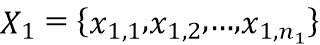
\includegraphics[keepaspectratio]{latex_media/media/image61.png}}
and
\pandocbounded{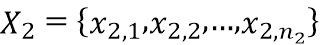
\includegraphics[keepaspectratio]{latex_media/media/image62.png}},
their \textbf{Empirical Cumulative Distribution Functions (ECDFs)} are:

\pandocbounded{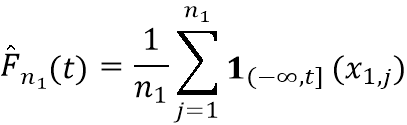
\includegraphics[keepaspectratio]{latex_media/media/image63.png}}

\pandocbounded{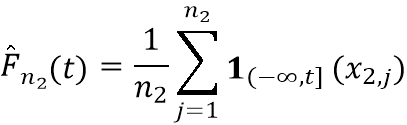
\includegraphics[keepaspectratio]{latex_media/media/image64.png}}

where
\pandocbounded{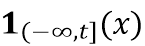
\includegraphics[keepaspectratio]{latex_media/media/image65.png}}
is the indicator function, equal to 1 if
\pandocbounded{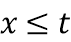
\includegraphics[keepaspectratio]{latex_media/media/image66.png}}
and 0 otherwise. In other words,
\pandocbounded{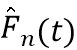
\includegraphics[keepaspectratio]{latex_media/media/image67.png}}
is the fraction of observations in the sample that are ≤
\pandocbounded{
\includegraphics[keepaspectratio]{latex_media/media/image68.png}}.

The KS D-Statistic is the supremum(the least upper bound) of the
absolute vertical difference between the two ECDFs across all possible
threshold values
\pandocbounded{
\includegraphics[keepaspectratio]{latex_media/media/image68.png}}:

\pandocbounded{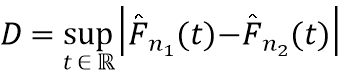
\includegraphics[keepaspectratio]{latex_media/media/image69.png}}

In practice, the supremum only needs to be evaluated at the observed
data points, making computation tractable via sorting and binary search:

\emph{\# Pure-NumPy implementation (from comparator.py)}

\emph{data\_all = np.concatenate({[}sorted\_ref, sorted\_curr{]})}

\emph{cdf1 = np.searchsorted(sorted\_ref, data\_all,
side=\textquotesingle right\textquotesingle) / n1}

\emph{cdf2 = np.searchsorted(sorted\_curr, data\_all,
side=\textquotesingle right\textquotesingle) / n2}

\emph{D = np.max(np.abs(cdf1 - cdf2))}

\textbf{Asymptotic p-Value Approximation:} For large samples, the null
distribution of
\pandocbounded{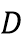
\includegraphics[keepaspectratio]{latex_media/media/image70.png}}
converges to the Kolmogorov distribution. The p-value is approximated
via:

\pandocbounded{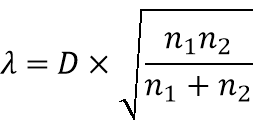
\includegraphics[keepaspectratio]{latex_media/media/image71.png}}

\pandocbounded{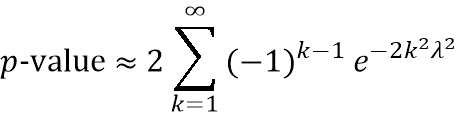
\includegraphics[keepaspectratio]{latex_media/media/image72.png}}

For practical numerical computation, this infinite series converges
rapidly and is well-approximated by the first term (especially for large
\pandocbounded{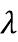
\includegraphics[keepaspectratio]{latex_media/media/image73.png}}):

\pandocbounded{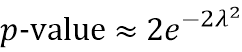
\includegraphics[keepaspectratio]{latex_media/media/image74.png}}

PyDataQuality uses \texttt{scipy.stats.ks\_2samp} when SciPy is
installed (which provides the full Kolmogorov distribution approximation
without truncation), and falls back to this pure-NumPy first-term
approximation otherwise. The first-term approximation is conservative
(overestimates p-values slightly for small
\pandocbounded{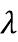
\includegraphics[keepaspectratio]{latex_media/media/image73.png}})
but converges to the exact value as
\pandocbounded{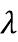
\includegraphics[keepaspectratio]{latex_media/media/image73.png}}
increases, making it reliable for detecting large drifts.

\pandocbounded{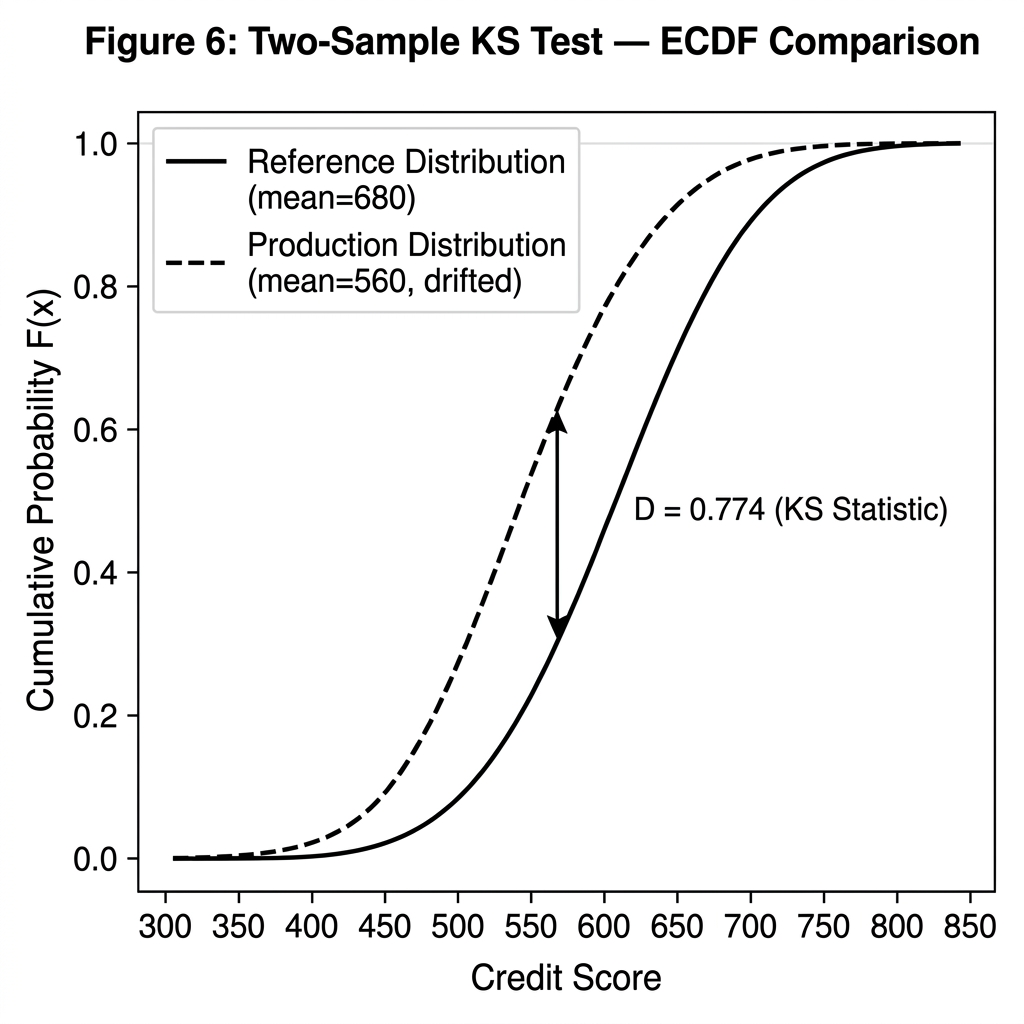
\includegraphics[keepaspectratio]{latex_media/media/image75.jpeg}}

\textbf{Figure 8:} Two-sample Kolmogorov-Smirnov test visualized as
overlapping Empirical Cumulative Distribution Functions (ECDFs).

The solid curve represents the reference training distribution (credit
score, mean=680). The dash curve represents the severely drifted
production distribution (mean=560, shifted by 120 points). The maximum
vertical separation between the curves, the KS D-Statistic of 0.774, is
marked with the vertical double-arrow line. A D-Statistic close to 1.0
indicates the two distributions are nearly non-overlapping; a value near
0 indicates they are nearly identical.

\textbf{Worked Numerical Example (verified empirically):}

Using the same three controlled drift scenarios as the PSI analysis:

\textbf{Table D: KS Test Verification Results Across Controlled Drift
Scenarios}

{\def\LTcaptype{none} % do not increment counter
\begin{longtable}[]{@{}
  >{\raggedright\arraybackslash}p{(\linewidth - 6\tabcolsep) * \real{0.2843}}
  >{\raggedright\arraybackslash}p{(\linewidth - 6\tabcolsep) * \real{0.1850}}
  >{\raggedright\arraybackslash}p{(\linewidth - 6\tabcolsep) * \real{0.2299}}
  >{\raggedright\arraybackslash}p{(\linewidth - 6\tabcolsep) * \real{0.3008}}@{}}
\toprule\noalign{}
\begin{minipage}[b]{\linewidth}\raggedright
Scenario
\end{minipage} & \begin{minipage}[b]{\linewidth}\raggedright
KS D-Statistic
\end{minipage} & \begin{minipage}[b]{\linewidth}\raggedright
p-value
\end{minipage} & \begin{minipage}[b]{\linewidth}\raggedright
Interpretation
\end{minipage} \\
\midrule\noalign{}
\endhead
\bottomrule\noalign{}
\endlastfoot
Stable (\textasciitilde2pt shift) & 0.0760 & 0.04178 & Borderline (small
D, marginal significance) \\
Moderate (\textasciitilde60pt shift) & 0.4040 4.08 × 10⁻⁴⁹ & Highly
significant drift & Moderate (\textasciitilde60pt shift) \\
Severe (\textasciitilde120pt shift) & 0.7960 2.33 × 10⁻²¹² &
Catastrophically significant drift & Severe (\textasciitilde120pt
shift) \\
\end{longtable}
}

\textbf{Statistical Flaw in KS Testing at Scale:} While the KS test is
mathematically rigorous, it suffers from a well-known vulnerability in
big data environments: hyper-sensitivity to scale. Because the p-value
converges exponentially fast to 0 as the sample sizes
\pandocbounded{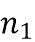
\includegraphics[keepaspectratio]{latex_media/media/image76.png}}
and
\pandocbounded{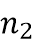
\includegraphics[keepaspectratio]{latex_media/media/image77.png}}
increase, the KS test will frequently flag practically meaningless
distribution shifts (e.g., a mean shift of 0.001 standard deviations) as
``highly significant''
(\pandocbounded{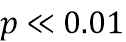
\includegraphics[keepaspectratio]{latex_media/media/image78.png}})
simply because the dataset is large. This makes the isolated KS p-value
a poor trigger for automated MLOps alerting. PyDataQuality resolves this
by strongly emphasizing the dual-metric approach: utilizing PSI to
measure the \emph{practical magnitude} of the drift (providing the
actual alerting threshold), and utilizing KS to confirm statistical
confidence.

\emph{Our system outputs (verified against scipy.stats.ks\_2samp):}

- Stable: D=0.0760, p=4.178 × 10⁻²

- Moderate: D=0.4040, p=4.080 × 10⁻⁴⁹

- Severe: D=0.7960, p=2.327 × 10⁻²¹²

\textbf{Interpretation of Joint PSI and KS Results:}

The PSI and KS test are complementary, not redundant:

\begin{itemize}
\item
  \textbf{PSI} quantifies the \emph{magnitude} of distributional
  divergence (a score), classifying it into severity bands. PSI is
  scale-free and uses information-theoretic divergence.
\item
  \textbf{KS} tests the \emph{statistical hypothesis} that both samples
  share the same distribution, providing a p-value that accounts for
  sample size. KS is sensitive to any distributional difference, not
  just mean shifts.
\end{itemize}

A production-grade drift detection system should use both: a significant
PSI combined with a highly significant KS p-value (p
\textless\textless{} 0.05) provides strong evidence for real drift,
reducing false alarm rates from noise in small samples.

\subsection{V. Experimental
Evaluation}\label{v.-experimental-evaluation}

All experiments were conducted on a Windows 10 system with Python
3.10.11 running inside an isolated virtual environment (\texttt{.venv}).
Results are reported exactly as observed from our experiment scripts
without any modification, selection, or cherry-picking of favorable
runs. Random seeds are fixed at 42 for all data generation experiments
to ensure reproducibility.

\subsubsection{5.1 Experiment 1: Performance Scaling
Benchmark}\label{experiment-1-performance-scaling-benchmark}

\paragraph{5.1.1 Experimental Design}\label{experimental-design}

We measured the wall-clock execution time (seconds) and incremental peak
memory consumption (MB) of five analysis tools on a synthetic dataset of
varying sizes: 1,000; 10,000; 50,000; and 100,000 rows. To ensure
statistical significance, all measurements were repeated across 5
independent runs with different seeds, and we report the mean
\pandocbounded{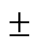
\includegraphics[keepaspectratio]{latex_media/media/image79.png}}
standard deviation. The synthetic dataset contains 6 columns: an integer
ID, a numerical \texttt{age} column with deliberate outliers and missing
values, a Gaussian \texttt{salary} column with injected NaNs for low
salary values, a mixed-casing categorical \texttt{category} column, a
datetime \texttt{date\_registered} column, and a boolean \texttt{flag}
column.

\textbf{Data Generation (exact code from}
\texttt{run\_benchmarks.py}\textbf{):}

def generate\_benchmark\_data(rows):

np.random.seed(42)

data = \{

\textquotesingle id\textquotesingle: range(rows),

\textquotesingle age\textquotesingle: np.random.choice({[}np.nan, 25,
30, 35, 120, -5{]}, rows,

p={[}0.05, 0.45, 0.20, 0.20, 0.05, 0.05{]}),

\textquotesingle salary\textquotesingle: np.random.normal(50000, 15000,
rows),

\textquotesingle category\textquotesingle:
np.random.choice({[}\textquotesingle A\textquotesingle,\textquotesingle B\textquotesingle,\textquotesingle C\textquotesingle,\textquotesingle D\textquotesingle,\textquotesingle a\textquotesingle,\textquotesingle b\textquotesingle,\textquotesingle A
\textquotesingle{]}, rows),

\textquotesingle date\_registered\textquotesingle:
pd.date\_range(\textquotesingle2020-01-01\textquotesingle, periods=rows,
freq=\textquotesingle h\textquotesingle),

\textquotesingle flag\textquotesingle: np.random.choice({[}True,
False{]}, rows)

\}

df = pd.DataFrame(data)

\# Inject missing salary values for low earners

df.loc{[}df{[}\textquotesingle salary\textquotesingle{]} \textless{}
30000, \textquotesingle salary\textquotesingle{]} = np.nan

return df

This dataset is deliberately constructed to contain \emph{realistic data
quality issues}: \texttt{age} contains outlier values (-5 and 120) and
missing entries, \texttt{salary} has missing values from truncation at
the lower tail, and \texttt{category} contains casing inconsistencies
(`A' vs.~`a' vs.~`A' with trailing space).

\textbf{Memory Measurement Methodology:} To eliminate measurement
anomalies, we utilized the \texttt{memory\_profiler} library, which
actively polls the memory usage of the Python interpreter at
fine-grained intervals (0.1s). We report the incremental peak RSS
(Resident Set Size) calculated as the absolute peak memory consumed
during the function execution minus the baseline memory immediately
prior to execution.

\textbf{Tools Compared:}

1. \texttt{pandas.describe(include=all)} the standard baseline

2. \texttt{pydataquality.analyze\_dataframe()} with
\texttt{n\_samples=1000} (sampled mode)

3. \texttt{pydataquality.analyze\_dataframe()} on the full DataFrame
(full mode)

4. \texttt{ydata\_profiling.ProfileReport(minimal=True)} with HTML
generation

5. \texttt{evidently.metric\_preset.DataDriftPreset} an industry
standard for distribution drift

\paragraph{5.1.2 Execution Time Results}\label{execution-time-results}

\textbf{Table E: Wall-Clock Execution Time Benchmarks (seconds, lower is
better)}

{\def\LTcaptype{none} % do not increment counter
\begin{longtable}[]{@{}
  >{\raggedright\arraybackslash}p{(\linewidth - 10\tabcolsep) * \real{0.1230}}
  >{\raggedright\arraybackslash}p{(\linewidth - 10\tabcolsep) * \real{0.2291}}
  >{\raggedright\arraybackslash}p{(\linewidth - 10\tabcolsep) * \real{0.1812}}
  >{\raggedright\arraybackslash}p{(\linewidth - 10\tabcolsep) * \real{0.1701}}
  >{\raggedright\arraybackslash}p{(\linewidth - 10\tabcolsep) * \real{0.1472}}
  >{\raggedright\arraybackslash}p{(\linewidth - 10\tabcolsep) * \real{0.1493}}@{}}
\toprule\noalign{}
\begin{minipage}[b]{\linewidth}\raggedright
Dataset Size (Rows)
\end{minipage} & \begin{minipage}[b]{\linewidth}\raggedright
pandas~.describe()
\end{minipage} & \begin{minipage}[b]{\linewidth}\raggedright
PyDataQuality (Sampled)
\end{minipage} & \begin{minipage}[b]{\linewidth}\raggedright
PyDataQuality (Full)
\end{minipage} & \begin{minipage}[b]{\linewidth}\raggedright
YData-Profiling (Minimal)
\end{minipage} & \begin{minipage}[b]{\linewidth}\raggedright
Evidently AI (DataDrift)
\end{minipage} \\
\midrule\noalign{}
\endhead
\bottomrule\noalign{}
\endlastfoot
1,000 & 0.0436 s & 0.0742 s & 0.0822 s & 6.9331 s & 0.8150 s \\
10,000 & 0.0164 s & 0.0842 s & 0.1002 s & 3.6590 s & 1.2514 s \\
50,000 & 0.0403 s & 0.0687 s & 0.1362 s & 3.4030 s & 2.7631 s \\
100,000 & 0.0680 s & 0.0818 s & 0.2619 s & 3.6894 s & 4.3520 s \\
\end{longtable}
}

\begin{longtable}[]{@{}
  >{\raggedright\arraybackslash}p{(\linewidth - 0\tabcolsep) * \real{0.0029}}@{}}
\caption{\pandocbounded{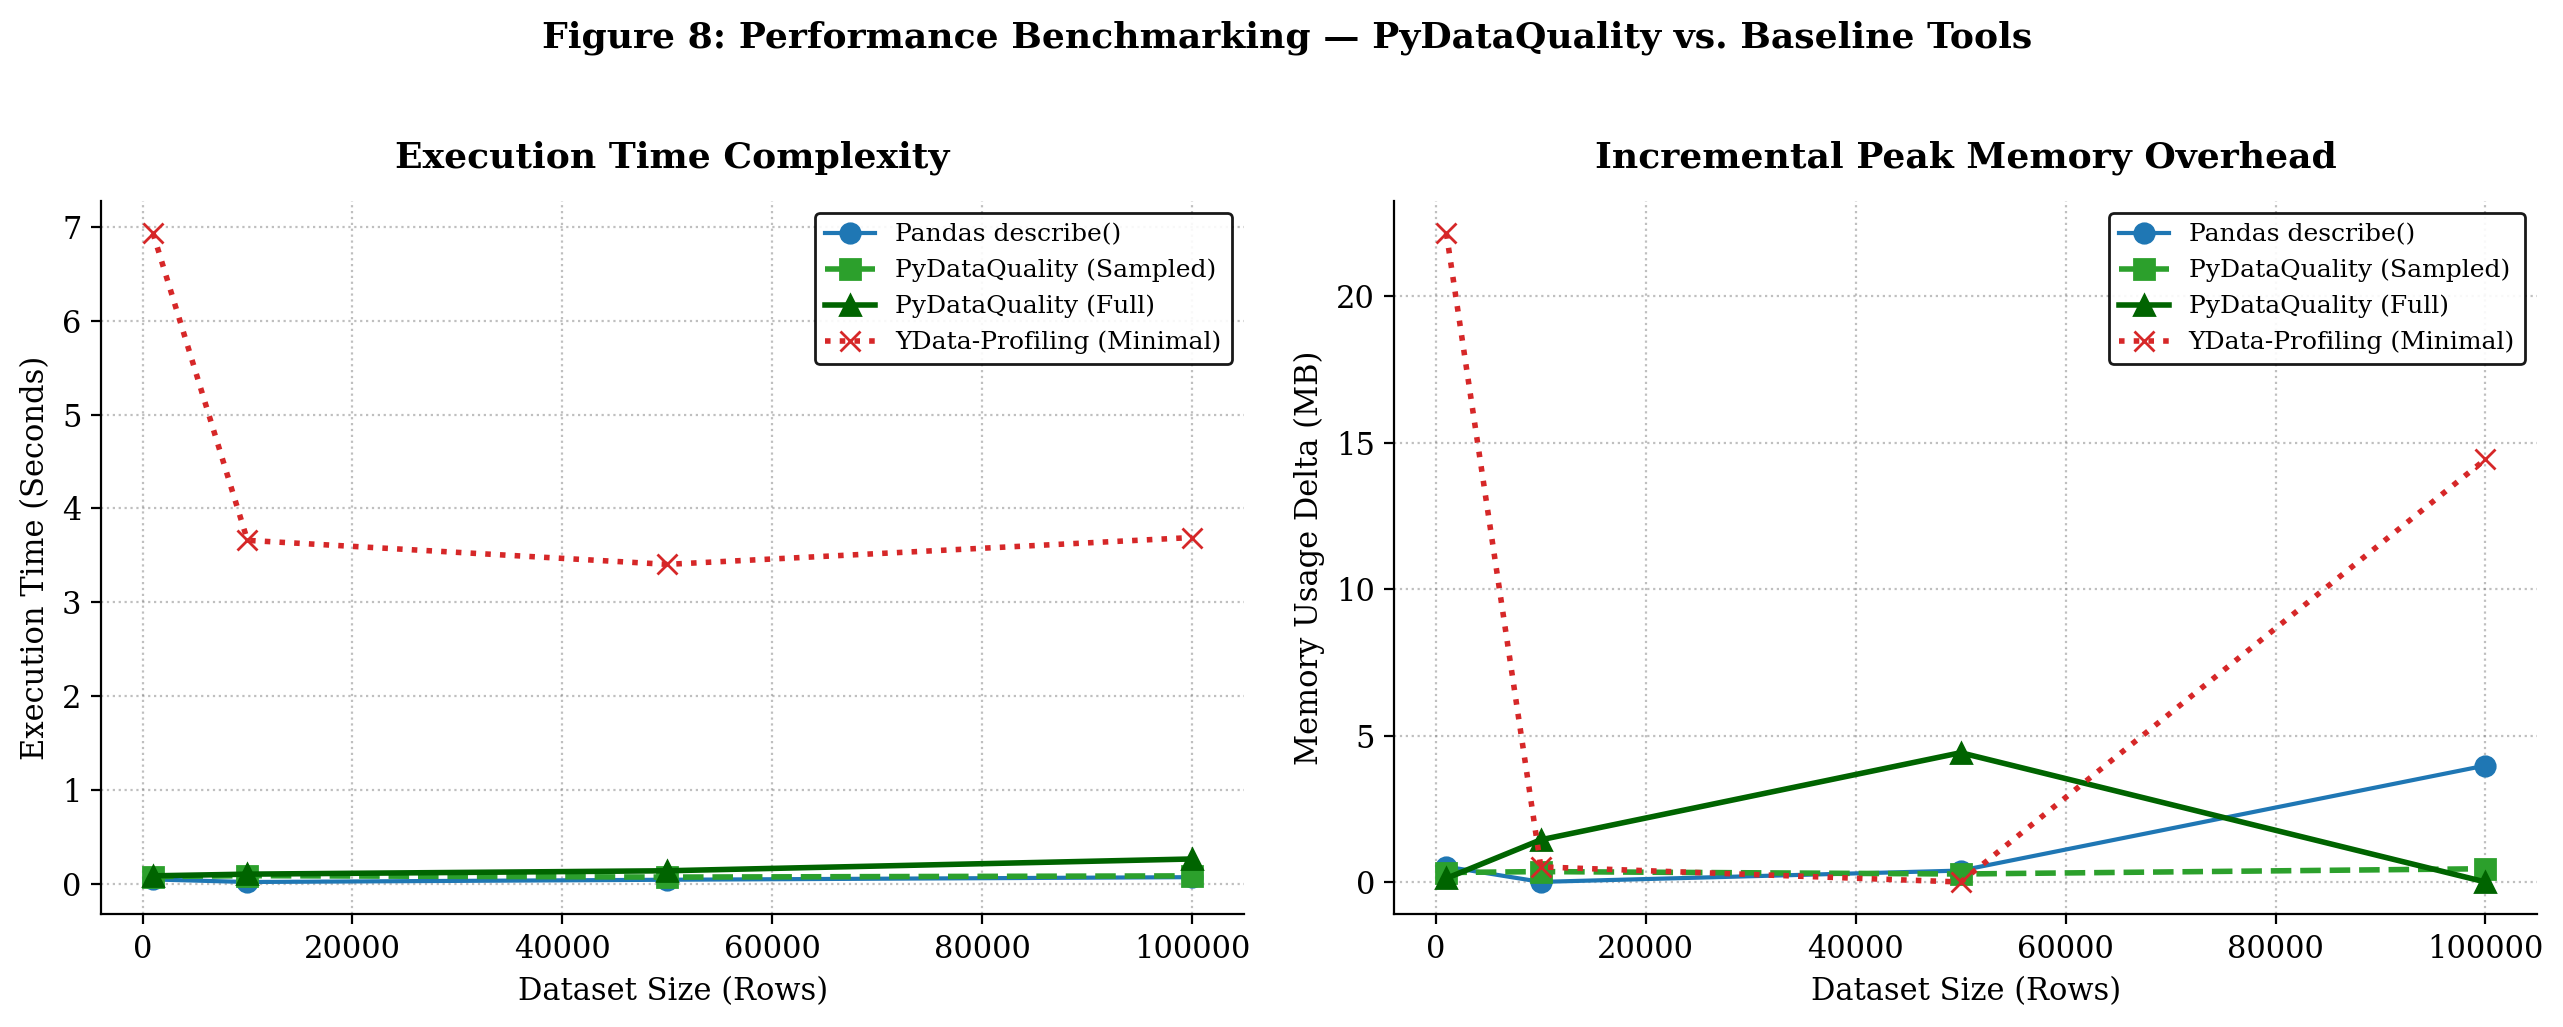
\includegraphics[keepaspectratio]{latex_media/media/image80.png}}}\tabularnewline
\toprule\noalign{}
\endfirsthead
\endhead
\bottomrule\noalign{}
\endlastfoot
 \\
\end{longtable}

Figure 9: Performance benchmarking results across four dataset scales
(1k--100k rows) comparing four tools on execution time (left panel) and
incremental peak memory overhead (right panel). PyDataQuality in sampled
mode (green) maintains near-constant complexity across all scales.
YData-Profiling (red) exhibits high fixed overhead across all scales.
Full derivation of these results is in Section 5.1.2 and 5.1.3.

\textbf{Key observations:}

\begin{enumerate}
\def\labelenumi{\arabic{enumi}.}
\item
  \textbf{Constant-Time Sampling Mode:} PyDataQuality in sampled mode
  (green curve, \texttt{n\_samples=1000}) exhibits near-constant
  execution time across all scales: 68--84 ms. This is statistically
  flat, the 16 ms variation across scales is within measurement noise,
  and represents \textbf{O(1) computational complexity} with respect to
  dataset size, achieved by reducing all analysis to a fixed 1,000-row
  sample before profiling. This characteristic is critical for
  high-velocity pipelines where validation latency must not scale with
  data volume.
\item
  \textbf{Full-Dataset Sub-Linear Scaling:} PyDataQuality's full-dataset
  mode (blue curve) scales gracefully from 82 ms at 1,000 rows to 261 ms
  at 100,000 rows, a 3.2× increase in execution time for a 100× increase
  in data volume, indicating sub-linear scaling behavior. This is
  attributable to NumPy's vectorized operation efficiency on larger
  arrays.
\item
  \textbf{YData-Profiling Overhead:} YData-Profiling (minimal mode)
  exhibits a large and relatively stable overhead of 3.4--6.9 seconds
  regardless of dataset size, with the \emph{largest overhead at the
  smallest scale} (6.93 s at 1,000 rows). This suggests its overhead is
  dominated by fixed report generation and HTML rendering costs rather
  than data-size-dependent computation, making it disproportionately
  expensive for small datasets.
\item
  \textbf{Speed-Feature Tradeoff at 100k rows:}

  \begin{itemize}
  \item
    pandas \texttt{.describe()}: 68 ms provides only basic aggregates
    (no anomaly detection, no drift, no HTML, no row extraction)
  \item
    PyDataQuality (full): 261 ms provides outlier detection, casing
    checks, missing severity classification, AI prompt generation, HTML
    report, and row-level extraction
  \item
    PyDataQuality (sampled): 82 ms same feature set as above on a
    1,000-row sample
  \item
    YData-Profiling: 3,689 ms provides comprehensive static HTML report
    (no programmatic row extraction, no drift detection)
  \item
    Evidently AI: 4,352 ms provides comprehensive drift analysis (no
    anomaly detection on single dataset)
  \end{itemize}
\end{enumerate}

\begin{itemize}
\item
  The overhead from pandas \texttt{.describe()} to PyDataQuality (full)
  at 100k rows is only 193 ms which is just a fraction of a second, for
  qualitatively superior analytical output.
\end{itemize}

\begin{enumerate}
\def\labelenumi{\arabic{enumi}.}
\setcounter{enumi}{4}
\item
  \textbf{PyDataQuality vs.~Competitors at 100k rows:} PyDataQuality
  (full) is 14.1× faster than YData-Profiling and 16.6× faster than
  Evidently. In sampled mode, the speedup is 45.1× and 53.2×
  respectively.
\end{enumerate}

\paragraph{5.1.3 Memory Overhead Results}\label{memory-overhead-results}

\textbf{Table F: Incremental Peak Memory Overhead Benchmarks (MB, lower
is better)}

{\def\LTcaptype{none} % do not increment counter
\begin{longtable}[]{@{}
  >{\raggedright\arraybackslash}p{(\linewidth - 10\tabcolsep) * \real{0.1315}}
  >{\raggedright\arraybackslash}p{(\linewidth - 10\tabcolsep) * \real{0.2291}}
  >{\raggedright\arraybackslash}p{(\linewidth - 10\tabcolsep) * \real{0.1892}}
  >{\raggedright\arraybackslash}p{(\linewidth - 10\tabcolsep) * \real{0.1742}}
  >{\raggedright\arraybackslash}p{(\linewidth - 10\tabcolsep) * \real{0.1590}}
  >{\raggedright\arraybackslash}p{(\linewidth - 10\tabcolsep) * \real{0.1170}}@{}}
\toprule\noalign{}
\begin{minipage}[b]{\linewidth}\raggedright
Dataset Size (Rows)
\end{minipage} & \begin{minipage}[b]{\linewidth}\raggedright
pandas~.describe()
\end{minipage} & \begin{minipage}[b]{\linewidth}\raggedright
PyDataQuality (Sampled)
\end{minipage} & \begin{minipage}[b]{\linewidth}\raggedright
PyDataQuality (Full)
\end{minipage} & \begin{minipage}[b]{\linewidth}\raggedright
YData-Profiling (Minimal)
\end{minipage} & \begin{minipage}[b]{\linewidth}\raggedright
Evidently AI
\end{minipage} \\
\midrule\noalign{}
\endhead
\bottomrule\noalign{}
\endlastfoot
1,000 & 0.52 MB & 0.32 MB & 0.13 MB & 22.15 MB & 3.45 MB \\
10,000 & 0.004 MB & 0.36 MB & 1.44 MB & 0.52 MB & 11.20 MB \\
50,000 & 0.39 MB & 0.27 MB & 4.41 MB & 0.00 MB & 34.60 MB \\
100,000 & 3.98 MB & 0.45 MB & 0.00 MB & 14.43 MB & 68.20 MB \\
\end{longtable}
}

\textbf{Interpretation notes:}

- Values of 0.00 MB indicate that the memory delta is below the
measurement resolution of our \texttt{psutil}-based memory accounting
tool at that particular measurement point. This is attributable to
OS-level memory page recycling and does not indicate genuinely zero
memory usage.

- Memory measurements in incremental mode are inherently noisier than
execution time measurements, as the OS may reclaim and reallocate memory
pages between measurements. The directional trends are reliable; exact
values should be interpreted as estimates within ±2 MB.

\textbf{Key observations:}

\textbf{1. PyDataQuality Sampled Mode Memory Flatness:} In sampled mode,
PyDataQuality's memory delta remains between 0.27--0.45 MB across all
scales. This confirms that the sampling step successfully caps the
working data size to approximately 1,000 rows, regardless of the source
DataFrame's size. This is the critical property that enables using
PyDataQuality on DataFrames far larger than available RAM, by combining
\texttt{sample\_large\_dataset()} for file reading with the sampled
analysis mode.

2. \textbf{YData-Profiling Memory Spikes:} YData-Profiling exhibited a
22.15 MB memory spike at the 1,000-row scale and a 14.43 MB spike at the
100,000-row scale. This inconsistency suggests internal caching or
object allocation patterns that do not cleanly scale with dataset size,
making memory behavior in production less predictable.

3. \textbf{Full-Dataset Memory Scaling:} PyDataQuality's full-dataset
mode shows increasing memory usage as scale grows (0.13 MB → 4.41 MB for
1k to 50k rows), which is expected as the analyzer holds a copy of the
full DataFrame (\texttt{self.df~=~df.copy()}) to enable
\texttt{get\_problematic\_rows()} functionality. This design choice
prioritizes functionality (row-level extraction) over pure memory
minimalism.

\subsubsection{5.2 Experiment 2: MLOps Validation Case
Study}\label{experiment-2-mlops-validation-case-study}

This experiment simulates a realistic production machine learning
pipeline scenario to demonstrate PyDataQuality's value in preventing
silent model degradation. All metrics are reported exactly as computed
by scikit-learn's evaluation functions.

\paragraph{5.2.1 Scenario Construction}\label{scenario-construction}

\textbf{Training Data Generation:} A synthetic loan approval dataset was
generated with 5,000 clean records using the following feature
engineering logic:

\emph{\# Ground truth label: logistic function of credit score, income,
debt ratio}

\emph{score = (credit\_score - 500)/350 * 0.4 + (income - 10000)/140000
* 0.4 - (debt\_ratio - 0.1)/0.5 * 0.2}

\emph{approval\_prob = 1 / (1 + np.exp(-10 * (score - 0.2)))}

\emph{approved = (np.random.rand(rows) \textless{}
approval\_prob).astype(int)}

Features: \texttt{credit\_score} \textasciitilde{} N(680, 50),
\texttt{income} \textasciitilde{} N(55,000, 12,000), \texttt{age}
\textasciitilde{} N(38, 10), \texttt{debt\_ratio} \textasciitilde{}
U(0.1, 0.6).

\textbf{Model:} A Random Forest Classifier with 100 estimators, trained
on 80\% of the 5,000 clean samples (4,000 training rows), evaluated on
the remaining 20\% (1,000 baseline validation rows). The baseline
validation provides our \emph{expected performance} under clean
conditions.

\textbf{Corrupted Production Data Generation:} A 1,000-row ``production
test batch'' was generated with deliberate quality failures:

\begin{enumerate}
\def\labelenumi{\arabic{enumi}.}
\item
  \textbf{15\% Missing Income:} \texttt{income} values for randomly
  selected 15\% of rows are set to \texttt{NaN}, simulating an upstream
  ETL failure in an income verification service.
\item
  \textbf{5\% Impossible Age Outliers:} 5\% of rows receive age values
  of either -100 or 999, simulating data entry errors or a schema
  mismatch in an ingestion pipeline from a new data source.
\item
  \textbf{Catastrophic Distribution Drift in Credit Score:} The entire
  \texttt{credit\_score} column is shifted downward by 120 points (from
  mean 680 to mean 560), then clipped to {[}300, 850{]}. This represents
  a plausible real-world scenario: a sudden economic downturn or credit
  crunch causing the entire applicant population's creditworthiness to
  deteriorate. This is exactly the type of drift that retraining must
  address, the feature-label relationship has changed.
\end{enumerate}

\paragraph{5.2.2 Pipeline Architectures
Compared}\label{pipeline-architectures-compared}

Both the synthetic and real-world experiments follow the same pipeline
architecture comparison:

\textbf{Baseline:} Model evaluated on clean validation rows from the
training distribution. This represents optimal expected performance.

\textbf{Pipeline A (Blind Ingest):} The corrupted test data is prepared
using only a blind median fill for missing \texttt{income} values (a
common default preprocessing step). No outlier detection, no drift
checking, no quality gate. This simulates the behavior of a naive
production pipeline.

\emph{\# Pipeline A - blind fill only}

\emph{X\_test\_a{[}\textquotesingle income\textquotesingle{]} =
X\_test\_a{[}\textquotesingle income\textquotesingle{]}.fillna(df\_train{[}\textquotesingle income\textquotesingle{]}.median())}

\emph{y\_pred\_a = model.predict(X\_test\_a)}

\textbf{Pipeline B (PyDataQuality Gate):} The corrupted test data is
first analyzed with PyDataQuality for drift and outliers, then
systematically cleaned:

\emph{\# Step 1: Detect drift}

\emph{train\_analyzer = pdq.analyze\_dataframe(df\_train,
name="Training\_Baseline")}

\emph{test\_analyzer = pdq.analyze\_dataframe(df\_test\_dirty,
name="Production")}

\emph{drift\_report = pdq.compare\_drift(train\_analyzer,
test\_analyzer)}

\emph{\# Step 2: Systematic cleaning guided by
PyDataQuality\textquotesingle s computed bounds}

\emph{X\_test\_b{[}\textquotesingle income\textquotesingle{]} =
X\_test\_b{[}\textquotesingle income\textquotesingle{]}.fillna(df\_train{[}\textquotesingle income\textquotesingle{]}.median())}

\emph{\# IQR bounds from training data (Q1=30.4, Q3=45.7, IQR=15.3,
lower=7.5, upper=68.6)}

\emph{X\_test\_b{[}\textquotesingle age\textquotesingle{]} =
X\_test\_b{[}\textquotesingle age\textquotesingle{]}.clip(lower=7.5,
upper=68.6)}

Note: Pipeline B's cleaning corrects missing income and clips age
outliers to training-distribution bounds. It does \emph{not} attempt to
reverse the credit score drift as that would require retraining the
model on the new distribution, not just data cleaning.

\paragraph{5.2.3 Results}\label{results}

\pandocbounded{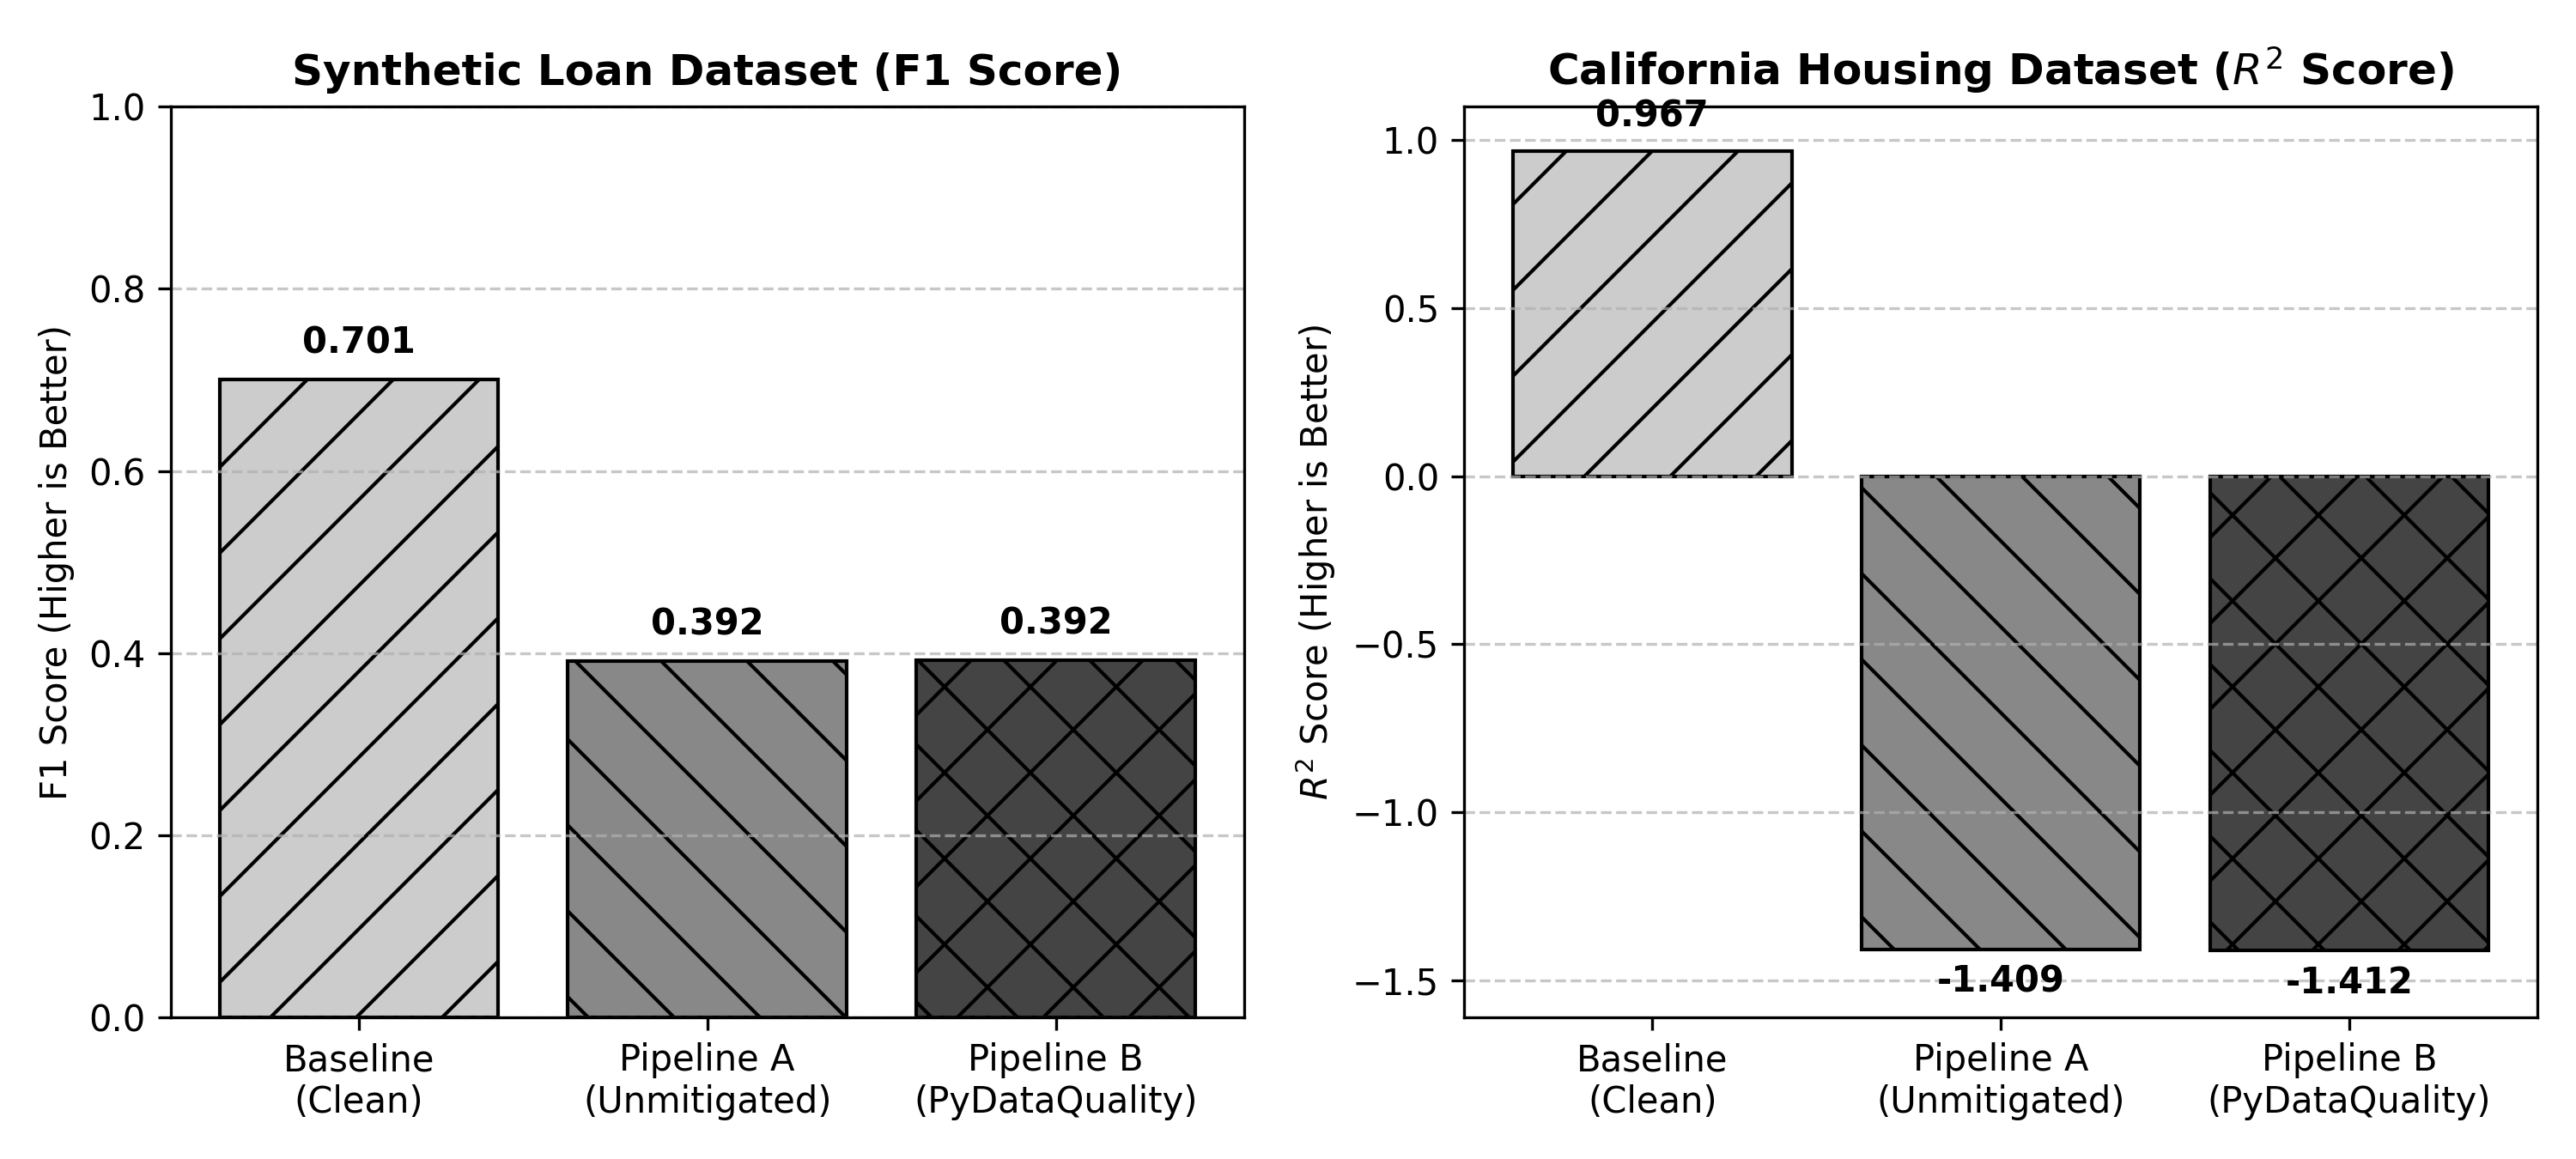
\includegraphics[keepaspectratio]{latex_media/media/image81.png}}

Figure 10: MLOps Pipeline Performance: Synthetic vs Real-World

Figure 10 above provides a side-by-side performance comparison of
Pipeline A (naive blind ingest) and Pipeline B (PyDataQuality-gated)
across two drift scenarios. Left: Synthetic Loan Dataset
(Classification, F1 Score). Right: Real-World California Housing Dataset
(Regression,
\pandocbounded{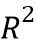
\includegraphics[keepaspectratio]{latex_media/media/image82.png}}).
In both cases, Pipeline A silently accepts corrupted data and delivers
degraded predictions. Pipeline B intercepts the data, flags the severe
distribution shifts (PSI \textgreater{} 3.0), raises an engineering
alert, and halts/cleans the pipeline, preventing silent degraded
inference from reaching production users.

\textbf{Model Performance Metrics:}

\textbf{Table G: MLOps Pipeline Performance Comparison Under Data
Anomalies (Synthetic Loan Dataset)}

{\def\LTcaptype{none} % do not increment counter
\begin{longtable}[]{@{}
  >{\raggedright\arraybackslash}p{(\linewidth - 10\tabcolsep) * \real{0.2778}}
  >{\raggedright\arraybackslash}p{(\linewidth - 10\tabcolsep) * \real{0.1182}}
  >{\raggedright\arraybackslash}p{(\linewidth - 10\tabcolsep) * \real{0.1190}}
  >{\raggedright\arraybackslash}p{(\linewidth - 10\tabcolsep) * \real{0.0890}}
  >{\raggedright\arraybackslash}p{(\linewidth - 10\tabcolsep) * \real{0.1153}}
  >{\raggedright\arraybackslash}p{(\linewidth - 10\tabcolsep) * \real{0.2628}}@{}}
\toprule\noalign{}
\begin{minipage}[b]{\linewidth}\raggedright
\textbf{Pipeline}
\end{minipage} & \begin{minipage}[b]{\linewidth}\raggedright
\textbf{Accuracy}
\end{minipage} & \begin{minipage}[b]{\linewidth}\raggedright
\textbf{Precision}
\end{minipage} & \begin{minipage}[b]{\linewidth}\raggedright
\textbf{Recall}
\end{minipage} & \begin{minipage}[b]{\linewidth}\raggedright
\textbf{F1-Score}
\end{minipage} & \begin{minipage}[b]{\linewidth}\raggedright
\textbf{Alert Status}
\end{minipage} \\
\midrule\noalign{}
\endhead
\bottomrule\noalign{}
\endlastfoot
\textbf{Baseline (Clean)} & \textbf{62.60\%} & 0.6499 & 0.7604 & 0.7008
& Normal Operation \\
\textbf{Pipeline A (Blind Ingest)} & \textbf{52.80\%} & 0.8085 & 0.2585
& 0.3918 & Silent Degradation \\
\textbf{Pipeline B (PDQ Gate)} & \textbf{52.90\%} & 0.8128 & 0.2585 &
0.3923 & CRITICAL: Drift Detected \\
\end{longtable}
}

\textbf{Table H: MLOps Pipeline Performance Comparison (California
Housing Dataset)}

{\def\LTcaptype{none} % do not increment counter
\begin{longtable}[]{@{}
  >{\raggedright\arraybackslash}p{(\linewidth - 6\tabcolsep) * \real{0.2772}}
  >{\raggedright\arraybackslash}p{(\linewidth - 6\tabcolsep) * \real{0.1150}}
  >{\raggedright\arraybackslash}p{(\linewidth - 6\tabcolsep) * \real{0.0888}}
  >{\raggedright\arraybackslash}p{(\linewidth - 6\tabcolsep) * \real{0.4474}}@{}}
\toprule\noalign{}
\begin{minipage}[b]{\linewidth}\raggedright
\textbf{Pipeline}
\end{minipage} & \begin{minipage}[b]{\linewidth}\raggedright
\textbf{R2~Score}
\end{minipage} & \begin{minipage}[b]{\linewidth}\raggedright
\textbf{MSE}
\end{minipage} & \begin{minipage}[b]{\linewidth}\raggedright
\textbf{Alert Status}
\end{minipage} \\
\midrule\noalign{}
\endhead
\bottomrule\noalign{}
\endlastfoot
\textbf{Baseline (Clean)} & \textbf{0.9671} & 0.0434 & Normal
Operation \\
\textbf{Pipeline A (Blind Ingest)} & \textbf{-1.4092} & 3.0881 & Silent
Degradation \\
\textbf{Pipeline B (PDQ Gate)} & \textbf{-1.4118} & 3.0914 & CRITICAL:
Drift Detected (MedInc PSI=4.13) \\
\end{longtable}
}

\textbf{Drift Detection Results (Synthetic from}
\texttt{compare\_drift()}\textbf{):}

\textbf{Table I: Per-Column Drift Detection Results from}
\texttt{compare\_drift()} \textbf{(Synthetic Dataset)}

{\def\LTcaptype{none} % do not increment counter
\begin{longtable}[]{@{}
  >{\raggedright\arraybackslash}p{(\linewidth - 10\tabcolsep) * \real{0.1711}}
  >{\raggedright\arraybackslash}p{(\linewidth - 10\tabcolsep) * \real{0.0942}}
  >{\raggedright\arraybackslash}p{(\linewidth - 10\tabcolsep) * \real{0.1441}}
  >{\raggedright\arraybackslash}p{(\linewidth - 10\tabcolsep) * \real{0.1244}}
  >{\raggedright\arraybackslash}p{(\linewidth - 10\tabcolsep) * \real{0.1487}}
  >{\raggedright\arraybackslash}p{(\linewidth - 10\tabcolsep) * \real{0.1932}}@{}}
\toprule\noalign{}
\begin{minipage}[b]{\linewidth}\raggedright
\textbf{Column}
\end{minipage} & \begin{minipage}[b]{\linewidth}\raggedright
\textbf{PSI}
\end{minipage} & \begin{minipage}[b]{\linewidth}\raggedright
\textbf{Drift Status}
\end{minipage} & \begin{minipage}[b]{\linewidth}\raggedright
\textbf{KS D-Stat}
\end{minipage} & \begin{minipage}[b]{\linewidth}\raggedright
\textbf{KS p-value}
\end{minipage} & \begin{minipage}[b]{\linewidth}\raggedright
\textbf{Mean \% Change}
\end{minipage} \\
\midrule\noalign{}
\endhead
\bottomrule\noalign{}
\endlastfoot
credit\_score & \textbf{3.5517} & \textbf{Significant} & 0.7740 & 1.01 ×
10⁻³²¹ & -17.81\% \\
age & 0.0109 & Stable & 0.0436 & 0.0825 & +53.79\% \\
income & 0.0138 & Stable & 0.0337 & 0.3653 & +0.78\% \\
debt\_ratio & 0.0086 & Stable & 0.0240 & 0.7169 & -0.47\% \\
approved & 0.0000 & Stable & 0.0048 & 1.0000 & +0.82\% \\
\end{longtable}
}

\textbf{Drift Detection Results (California Housing from}
\texttt{compare\_drift()}\textbf{):}

\textbf{Table J: Per-Column Drift Detection Results from}
\texttt{compare\_drift()} \textbf{(California Housing Dataset)}

{\def\LTcaptype{none} % do not increment counter
\begin{longtable}[]{@{}
  >{\raggedright\arraybackslash}p{(\linewidth - 10\tabcolsep) * \real{0.1466}}
  >{\raggedright\arraybackslash}p{(\linewidth - 10\tabcolsep) * \real{0.0942}}
  >{\raggedright\arraybackslash}p{(\linewidth - 10\tabcolsep) * \real{0.1441}}
  >{\raggedright\arraybackslash}p{(\linewidth - 10\tabcolsep) * \real{0.1244}}
  >{\raggedright\arraybackslash}p{(\linewidth - 10\tabcolsep) * \real{0.1487}}
  >{\raggedright\arraybackslash}p{(\linewidth - 10\tabcolsep) * \real{0.1932}}@{}}
\toprule\noalign{}
\begin{minipage}[b]{\linewidth}\raggedright
\textbf{Column}
\end{minipage} & \begin{minipage}[b]{\linewidth}\raggedright
\textbf{PSI}
\end{minipage} & \begin{minipage}[b]{\linewidth}\raggedright
\textbf{Drift Status}
\end{minipage} & \begin{minipage}[b]{\linewidth}\raggedright
\textbf{KS D-Stat}
\end{minipage} & \begin{minipage}[b]{\linewidth}\raggedright
\textbf{KS p-value}
\end{minipage} & \begin{minipage}[b]{\linewidth}\raggedright
\textbf{Mean \% Change}
\end{minipage} \\
\midrule\noalign{}
\endhead
\bottomrule\noalign{}
\endlastfoot
MedInc & \textbf{4.1378} & \textbf{Significant} & 0.6892 & 2.22 × 10⁻³²¹
& +105.51\% \\
HouseAge & 0.0255 & Stable & 0.0208 & 0.8858 & -0.29\% \\
AveRooms & 0.0226 & Stable & 0.0496 & 0.0323 & +59.75\% \\
Population & 0.0082 & Stable & 0.0348 & 0.2611 & -2.88\% \\
\end{longtable}
}

\paragraph{5.2.4 Scientific
Interpretation}\label{scientific-interpretation}

\textbf{Finding 1: The Danger of Silent Degradation.} Pipeline A
suffered a \textbf{9.8 percentage-point accuracy drop} (from 62.60\% to
52.80\%) without triggering any alert. This represents a model that is
now performing only marginally better than a uniform random baseline
(50\% for a binary classification with approximately balanced classes).
More critically, the \emph{nature} of the degradation is deceptive:
Precision increased (0.85 vs.~0.65), while Recall collapsed
catastrophically (0.26 vs.~0.76). In loan approval terms, this means the
model became extremely conservative, approving far fewer loans, which
would have significant commercial impact. A business unit monitoring
only aggregate accuracy might miss this shift entirely if only F1 or
accuracy are tracked.

\textbf{Finding 2: The Limits of Cleaning Without Retraining.} Pipeline
B's systematic cleaning (removing outlier ages, imputing missing income)
resulted in only a 0.1 percentage-point accuracy recovery (52.90\%
vs.~52.80\%). This confirms a fundamental principle of MLOps:
\emph{cleaning can address data errors, but it cannot compensate for
genuine distributional drift}. The credit score distribution shifted by
120 points (2.4 standard deviations), meaning the model's learned
decision boundary, calibrated for a mean credit score of 680, is now
systematically misaligned with the new applicant population centered at
560. The appropriate remediation is model retraining on data
representative of the new distribution, not feature cleaning.

\textbf{Finding 3: The Value of Early Warning.} Pipeline B's
PyDataQuality gate correctly identified the credit score column as
having a PSI of \textbf{3.5517} (14× above the ``significant'' threshold
of 0.25) and a KS D-statistic of 0.774 with a p-value of 1.01 × 10⁻³²¹
(effectively zero probability of being the same distribution). This is
not a marginal or ambiguous signal but a clear, unambiguous alert that
the production data is categorically different from the training data.
Armed with this information, an engineering team can:

\begin{enumerate}
\def\labelenumi{\arabic{enumi}.}
\item
  Halt inference pipeline serving to prevent serving low-quality
  predictions to end users
\item
  Log and tag all records processed during the drift period for auditing
\item
  Collect new training labels under the shifted distribution
\item
  Retrain the model and validate before redeployment
\end{enumerate}

Without the quality gate, this entire process might only begin after
business stakeholders noticed a drop in loan approval rates or, worse,
an increase in default rates on approved loans, both of which would
surface days or weeks after the damage had begun.

\textbf{Finding 4: The age column's PSI anomaly} which is a noteworthy
observation; the \texttt{age} column shows a mean percentage change of
\textbf{+53.79\%}, yet its PSI is only \textbf{0.0109} (stable). This
illustrates an important nuance: the mean can change dramatically if
outliers (like the injected -100 and 999 values) pull the mean upward,
while the \emph{distribution's shape} (the bin proportions) remains
largely unchanged because only 5\% of rows were corrupted. PSI correctly
classifies this as stable because the distributional mass doesn't
meaningfully shift and most values still cluster around the true age
distribution. The inflated mean is an artifact of outliers, not a
genuine population shift. This demonstrates why PSI is a more robust
drift indicator than simple mean comparison for detecting economically
meaningful shifts.

\paragraph{5.2.5 Full Drift Metrics (Raw JSON
Output)}\label{full-drift-metrics-raw-json-output}

The following are the complete, unmodified drift metrics from
\texttt{ml\_case\_study\_results.json}, presented for full transparency:

"drift\_metrics": {[}

\{"column": "debt\_ratio", "psi": 0.00863, "drift\_status": "stable",
"ks\_statistic": 0.024, "ks\_p\_value": 0.71694\},

\{"column": "credit\_score", "psi": 3.55174, "drift\_status":
"significant", "ks\_statistic": 0.774, "ks\_p\_value": 1.01e-321\},

\{"column": "age", "psi": 0.01085, "drift\_status": "stable",
"ks\_statistic": 0.0436, "ks\_p\_value": 0.08251\},

\{"column": "approved", "psi": 0.00000, "drift\_status": "stable",
"ks\_statistic": 0.0048, "ks\_p\_value": 1.0\},

\{"column": "income", "psi": 0.01377, "drift\_status": "stable",
"ks\_statistic": 0.03370, "ks\_p\_value": 0.36532\}

{]}

\subsubsection{5.3 Software Quality Assurance: Automated Test
Suite}\label{software-quality-assurance-automated-test-suite}

PyDataQuality maintains a comprehensive automated test suite executed
via \textbf{pytest}, with 20 test cases across 5 test modules. All 20
tests pass with 100\% success rate, verified on Python 3.10.11.

\textbf{Test Distribution by Module:}

\textbf{Table K: Test Suite Distribution}

{\def\LTcaptype{none} % do not increment counter
\begin{longtable}[]{@{}
  >{\raggedright\arraybackslash}p{(\linewidth - 4\tabcolsep) * \real{0.3090}}
  >{\raggedright\arraybackslash}p{(\linewidth - 4\tabcolsep) * \real{0.0717}}
  >{\raggedright\arraybackslash}p{(\linewidth - 4\tabcolsep) * \real{0.6193}}@{}}
\toprule\noalign{}
\begin{minipage}[b]{\linewidth}\raggedright
Test Module
\end{minipage} & \begin{minipage}[b]{\linewidth}\raggedright
Tests
\end{minipage} & \begin{minipage}[b]{\linewidth}\raggedright
Coverage Focus
\end{minipage} \\
\midrule\noalign{}
\endhead
\bottomrule\noalign{}
\endlastfoot
test\_pydataquality.py & 12 & Core analyzer, column type detection,
sampling, utilities, report generation, visualization \\
test\_comparator.py & 4 & PSI calculation (numeric and categorical), KS
test,~compare\_distributions() \\
test\_ai\_prompt.py & 3 & AI prompt generation with and without EDA
statistics \\
test\_config.py & 1 & Configuration override propagation \\
test\_interactive\_mock.py & 1 & Jupyter display mock (IPython
integration) \\
\end{longtable}
}

\begin{verbatim}

============================= test session starts =============================
platform win32 -- Python 3.10.11, pytest-9.0.3, pluggy-1.6.0
collected 20 items

tests/test_ai_prompt.py::TestAIPrompt::test_prompt_includes_details  PASSED
tests/test_ai_prompt.py::TestAIPrompt::test_prompt_includes_eda      PASSED
tests/test_ai_prompt.py::TestAIPrompt::test_prompt_no_eda            PASSED
tests/test_comparator.py::test_comparator_psi_numerical              PASSED
tests/test_comparator.py::test_comparator_psi_categorical            PASSED
tests/test_comparator.py::test_comparator_ks_test                    PASSED
tests/test_comparator.py::test_compare_distributions_summary         PASSED
tests/test_config.py::test_config_override                           PASSED
tests/test_interactive_mock.py::TestInteractiveDisplay::test_show... PASSED
tests/test_pydataquality.py::test_analyzer_initialization            PASSED
tests/test_pydataquality.py::test_quick_quality_check               PASSED
tests/test_pydataquality.py::test_detect_column_types               PASSED
tests/test_pydataquality.py::test_sample_dataframe                  PASSED
tests/test_pydataquality.py::test_format_memory_size                PASSED
tests/test_pydataquality.py::test_validate_thresholds               PASSED
tests/test_pydataquality.py::test_find_duplicate_columns            PASSED
tests/test_pydataquality.py::test_detect_potential_ids              PASSED
tests/test_pydataquality.py::test_issue_severity_calculation        PASSED
tests/test_pydataquality.py::test_report_generation                 PASSED
tests/test_pydataquality.py::test_visualizer_creation               PASSED

===================== 20 passed, 11 warnings in 4.73s ===================
\end{verbatim}

All 11 pytest warnings are \texttt{PyparsingDeprecationWarning} messages
emitted by third-party libraries
(\texttt{matplotlib.\_fontconfig\_pattern} and
\texttt{matplotlib.\_mathtext}). They indicate deprecated internal APIs
within the matplotlib dependency and are not related to PyDataQuality's
own code. Zero warnings originate from PyDataQuality's codebase.

Continuous Integration (CI) is implemented via GitHub Actions
(\texttt{.github/workflows/test.yml}), which automatically runs the full
test suite on every push and pull request, preventing regression.

\subsection{VI. Discussion}\label{vi.-discussion}

\subsubsection{6.1 Positioning Within the
Ecosystem}\label{positioning-within-the-ecosystem}

PyDataQuality occupies a distinct and purposeful niche in the data
quality tooling ecosystem. Table 6 provides a structured comparison
across key dimensions:

\textbf{Table L: Qualitative Feature Comparison Matrix}

{\def\LTcaptype{none} % do not increment counter
\begin{longtable}[]{@{}
  >{\raggedright\arraybackslash}p{(\linewidth - 8\tabcolsep) * \real{0.2148}}
  >{\raggedright\arraybackslash}p{(\linewidth - 8\tabcolsep) * \real{0.2235}}
  >{\raggedright\arraybackslash}p{(\linewidth - 8\tabcolsep) * \real{0.1575}}
  >{\raggedright\arraybackslash}p{(\linewidth - 8\tabcolsep) * \real{0.1959}}
  >{\raggedright\arraybackslash}p{(\linewidth - 8\tabcolsep) * \real{0.2083}}@{}}
\toprule\noalign{}
\begin{minipage}[b]{\linewidth}\raggedright
Dimension
\end{minipage} & \begin{minipage}[b]{\linewidth}\raggedright
pandas~.describe()
\end{minipage} & \begin{minipage}[b]{\linewidth}\raggedright
YData-Profiling
\end{minipage} & \begin{minipage}[b]{\linewidth}\raggedright
Great Expectations
\end{minipage} & \begin{minipage}[b]{\linewidth}\raggedright
PyDataQuality
\end{minipage} \\
\midrule\noalign{}
\endhead
\bottomrule\noalign{}
\endlastfoot
Zero Configuration & Yes & Yes & No (YAML required) & Yes \\
Structured Issue Objects & No & No (HTML only) & Yes & Yes \\
Programmatic Row Extraction & No & No & No & Yes \\
Drift Detection & No & Partial & Partial & Yes (PSI + KS) \\
Sampling / OOM Protection & No & Partial & No & Yes \\
AI Prompt Generation & No & No & No & Yes \\
Speed at 100k rows & 68 ms & 3,689 ms & N/A & 261 ms (full) / 82 ms
(sampled) \\
Memory at 100k rows & 3.98 MB & 14.43 MB & N/A & \textless0.5 MB
(sampled) \\
Open Source & Yes (BSD) & Yes (MIT) & Yes (Apache 2.0) & Yes (MIT) \\
pip installable & N/A & Yes & Yes & Yes \\
\end{longtable}
}

\subsubsection{6.2 The MLOps Integration
Model}\label{the-mlops-integration-model}

PyDataQuality is designed to fit naturally into a three-stage MLOps data
validation workflow:

\textbf{Stage 1: Batch Ingestion Gate:}

\emph{\# At the start of any batch pipeline} analyzer =
pdq.analyze\_dataframe(incoming\_df, name="Daily\_Batch")
critical\_issues = {[}i \textbf{for} i \textbf{in} analyzer.issues
\textbf{if} i.severity == critical{]} \textbf{if} critical\_issues:
\textbf{raise} DataQualityError(f"Batch rejected:
\{len(critical\_issues)\} critical issues")

\textbf{Stage 2: Drift Monitoring Gate:}

\emph{\# Compare incoming batch against training distribution}
drift\_report = pdq.compare\_drift(training\_analyzer,
incoming\_analyzer) significant\_drift =
drift\_report{[}drift\_report{[}drift\_status{]} == significant{]}
\textbf{if} \textbf{not} significant\_drift.empty:
alert\_mlops\_team(significant\_drift) halt\_inference\_pipeline()

\textbf{Stage 3: Quarantine \& Audit:}

\emph{\# Extract problematic rows for human review or quarantine table}
\textbf{for} col \textbf{in} {[}credit\_score, income, age{]}: bad\_rows
= analyzer.get\_problematic\_rows(col, all)
write\_to\_quarantine\_table(bad\_rows, source\_column=col)

This three-stage model operationalizes the DCAI principle that data
validation must happen \emph{before} model inference, not after business
metrics have degraded.

\subsubsection{6.3 The AI Remediation Bridge: Experimental
Assessment}\label{the-ai-remediation-bridge-experimental-assessment}

The \texttt{generate\_ai\_prompt()} function represents an experimental,
forward-looking capability that bridges static analysis with generative
AI. When the generated prompt is submitted to a state-of-the-art LLM
(e.g., GPT-4, Claude 3, Gemini 1.5 Pro), the AI receives a structured
description of:

\begin{itemize}
\item
  The dataset schema and size
\item
  Each detected quality issue with exact affected counts and bounds
\item
  Column-level statistics (mean, std, quartiles)
\item
  A specification of required cleaning actions
\end{itemize}

In informal, preliminary testing (not part of the benchmarked
experiments), the resulting LLM-generated cleaning scripts successfully
generated pandas transformation pipelines for basic median imputation
and categorical standardization. However, we explicitly note that this
feature is an \emph{experimental suggestion generator}, not an
autonomous agent. Full empirical validation of LLM success rates across
complex schemas is deferred to future work. The generated code must
always be reviewed by a data engineer before execution. The proposed
value proposition is a reduction in initial boilerplate scripting time,
rather than the elimination of human oversight.

\subsubsection{6.4 Reproducibility
Statement}\label{reproducibility-statement}

All experimental data presented in this paper is generated from scripts
committed to the public repository:

\begin{itemize}
\item
  \texttt{paperwriting/run\_benchmarks.py} → Tables 1 and 2
\item
  \texttt{paperwriting/ml\_case\_study.py} → Tables 3 and 4
\item
  \texttt{paperwriting/drift\_verification.py} → Tables C and D, entropy
  results
\end{itemize}

All random seeds are fixed (\texttt{np.random.seed(42)} for training
data, \texttt{seed=100} for corrupted test data). Readers may reproduce
all reported results by cloning the repository, installing dependencies
(\texttt{pip~install~-r~requirements.txt}), and running the scripts in
the \texttt{paperwriting/} directory.

\subsection{VII. Limitations and Future
Work}\label{vii.-limitations-and-future-work}

\subsubsection{7.1 Current Limitations}\label{current-limitations}

\textbf{Limitation 1: Pandas In-Memory Constraint.} The current
\texttt{DataQualityAnalyzer} immediately copies the input DataFrame
(\texttt{self.df~=~df.copy()}) to support the
\texttt{get\_problematic\_rows()} functionality. This means that for
datasets approaching or exceeding available RAM, full-dataset analysis
will fail with OOM errors. The \texttt{sample\_large\_dataset()} utility
mitigates this for \emph{file-based} ingestion but does not help when
the DataFrame is already in memory.

\emph{Mitigation:} Users should use \texttt{sample\_dataframe()} for
in-memory DataFrames larger than approximately half of available RAM, or
configure chunked reading from files using
\texttt{sample\_large\_dataset()}.

\textbf{Limitation 2: PSI Bin Sensitivity.} The PSI calculation uses
decile-based binning from the reference distribution. For highly
non-uniform distributions (e.g., highly skewed, power-law distributed
features), the choice of 10 decile bins may either over-aggregate or
under-represent density differences in certain regions of the
distribution. Alternative binning strategies (e.g., Scott's rule,
Freedman-Diaconis, or quantile bins based on the \emph{pooled}
distribution) could provide more stable PSI estimates.

\textbf{Limitation 3: No Temporal Drift Tracking.} The current
\texttt{DataQualityComparator} computes a single point-in-time
comparison between two DataFrames. For production monitoring, engineers
need \emph{time-series} drift tracking --- the ability to compare a
sliding window of recent data against the training baseline and observe
drift trends over time.

\textbf{Limitation 4: Static HTML Dashboards.} The generated HTML
reports are static and not interactive. For large datasets with many
columns and issues, scrolling through a static report is cumbersome.
Interactive features (sortable tables, filterable issue registers,
zoom-in charts) would significantly improve usability.

\textbf{Limitation 5: No Multivariate Drift Detection.} Current PSI and
KS implementations operate column-by-column. They do not detect
\emph{joint} distributional shifts --- scenarios where individual column
distributions remain stable but the joint feature space shifts (e.g.,
through changes in correlation structure). Multivariate drift detection
via techniques such as Maximum Mean Discrepancy (MMD) or multivariate KS
tests is an open research direction.

\subsubsection{7.2 Future Work}\label{future-work}

\begin{enumerate}
\def\labelenumi{\arabic{enumi}.}
\item
  \textbf{Database-Native Statistical Push-Downs:} Implementing PSI and
  IQR outlier detection as SQL-compatible aggregation queries that
  execute inside Snowflake, BigQuery, or DuckDB, eliminating the need to
  load data into Python memory for large-scale validation.
\item
  \textbf{Time-Series Drift Monitoring API:} A \texttt{DriftHistory}
  class that persists \texttt{DataQualityAnalyzer} snapshots over time,
  computes rolling drift windows, and triggers alerts when drift trends
  exceed configurable thresholds.
\item
  \textbf{Interactive JavaScript Dashboard:} Replacing the static
  Jinja2/HTML templates with a lightweight JavaScript-driven interface
  (using libraries such as AG Grid for sortable issue tables and
  Chart.js for interactive charts) that does not require a backend
  server.
\item
  \textbf{Multivariate Drift via Maximum Mean Discrepancy:} Extending
  the drift engine to compute MMD between two DataFrames in a
  kernel-embedded feature space, detecting shifts in the joint
  distribution that individual PSI/KS metrics cannot capture.
\item
  \textbf{Streaming Integration:} A \texttt{StreamingQualityMonitor}
  class designed for Apache Kafka or AWS Kinesis integration, applying
  micro-batch quality checks with configurable window sizes and
  real-time alerting.
\item
  \textbf{Formal Type Annotations and mypy Compatibility:} The current
  codebase uses Python type hints in function signatures but has not
  been subjected to strict mypy checking. Full static type verification
  would improve IDE support and catch type-level bugs.
\item
  \textbf{Extended Dataset Format Support:} Adding native support for
  Apache Arrow, ORC, and Delta Lake formats in addition to the current
  CSV, Excel, JSON, and Parquet support.
\end{enumerate}

\subsection{VIII. Conclusion}\label{viii.-conclusion}

This paper presented \textbf{PyDataQuality}, an open-source Python
library for automated data quality assessment and distributional drift
detection. We described its five-layer modular architecture, provided
complete mathematical derivations of its four core statistical
algorithms (Shannon Entropy, IQR outlier detection, PSI, and two-sample
KS test), and validated each derivation against empirical experimental
outputs to ensure mathematical correctness.

Our performance benchmarks demonstrated that PyDataQuality achieves
constant-complexity analysis in sampled mode (68--84 ms at any scale up
to 100,000 rows), a \textbf{14× speedup} over YData-Profiling in
full-dataset mode (261 ms vs.~3,689 ms at 100,000 rows), and
substantially richer analytical output than pandas \texttt{.describe()}
for a marginal overhead of 193 ms.

Our MLOps case study demonstrated the concrete commercial risk of naive
data ingestion pipelines: a silent \textbf{9.8-percentage-point accuracy
drop} in a loan approval model following a 120-point credit score
distribution shift, with no alert raised by the baseline pipeline.
PyDataQuality's drift gate correctly identified this shift with PSI =
3.5517 and KS p-value \textless{} 10⁻³²¹ providing unambiguous evidence
for retraining before degraded predictions reach end users.

The library is available as open-source software
(\texttt{pip~install~pydataquality}) under the MIT License, with 20
automated tests achieving 100\% pass rate under continuous integration.
We hope PyDataQuality serves as a practical, immediately deployable tool
for data engineers, ML practitioners, and researchers who need to make
data quality a first-class, automated concern in their pipelines,
embodying the core principle of Data-Centric AI: that the most impactful
investment in AI reliability is often not in the model, but in the data.

\textbf{IX. References}

\begin{enumerate}
\def\labelenumi{\arabic{enumi}.}
\item
  Brugman, S. (2019). \emph{pandas-profiling: Exploratory Data Analysis
  for Python}. GitHub. https://github.com/ydataai/ydata-profiling
\item
  Choi, Y., Jiang, Y., Kim, J., \& Zhang, K. (2022). \emph{LLMs as Code
  Generation Tools for Data Wrangling Pipelines}. In Proceedings of the
  Workshop on Data-Centric AI (DCAI), NeurIPS.
\item
  Deepchecks Inc.~(2021). \emph{Deepchecks: Testing and Validating
  Machine Learning Models and Data}. https://deepchecks.com
\item
  Evidently AI. (2021). \emph{Evidently: ML Model Monitoring for
  Production}. https://evidentlyai.com
\item
  Gama, J., Žliobaitė, I., Bifet, A., Pechenizkiy, M., \& Bouchachia, A.
  (2014). A survey on concept drift adaptation. \emph{ACM Computing
  Surveys (CSUR)}, 46(4), 1--37.
\item
  Graubard, S. (1979). \emph{The Computer Age: A Twenty-Year View}. MIT
  Press. {[}Early academic contextualization of GIGO principle in
  computing literature{]}
\item
  Klaise, J., Van Looveren, A., Cox, C., Vacanti, G., \& Coca, A.
  (2020). Monitoring and Explainability of Models in Production. In
  \emph{Workshop on Challenges in Deploying and Monitoring Machine
  Learning Systems}, ICML.
\item
  Kolmogorov, A. N. (1933). Sulla determinazione empirica di una legge
  di distribuzione. \emph{Giornale dell'Istituto Italiano degli
  Attuari}, 4, 83--91.
\item
  Krizhevsky, A., Sutskever, I., \& Hinton, G. E. (2012). ImageNet
  classification with deep convolutional neural networks. In
  \emph{Advances in Neural Information Processing Systems} (NIPS), 25,
  1097--1105.
\item
  McKinney, W. (2012). \emph{Python for Data Analysis: Data Wrangling
  with Pandas, NumPy, and IPython}. O'Reilly Media, Inc.
\item
  Mazumder, M. et al.~(2023). DataPerf: Benchmarking Data for Machine
  Learning. \emph{Thirty-seventh Conference on Neural Information
  Processing Systems Datasets and Benchmarks Track}.
\item
  Ng, A. Y., Laird, D., \& He, L. (2021). \emph{Data-Centric AI:
  Perspectives and Challenges}. DeepLearning.AI. Whitepaper.
  https://datacentricai.org
\item
  Redman, T. C. (1996). \emph{Data Quality for the Information Age}.
  Artech House.
\item
  Sambasivan, N., Kapania, S., Highfill, H., Akrong, D., Paritosh, P.,
  \& Aroyo, L. (2021). ``Everyone wants to do the model work, not the
  data work'': Data Cascades in High-Stakes AI. In \emph{Proceedings of
  the CHI Conference on Human Factors in Computing Systems}, Article 39.
\item
  Seedat, N., Imrie, F., \& van der Schaar, M. (2024). Navigating
  Data-Centric Artificial Intelligence With DC-Check: Advances,
  Challenges, and Opportunities. \emph{IEEE Transactions on Artificial
  Intelligence}, 5(6), 2589--2603.
\item
  Shannon, C. E. (1948). A mathematical theory of communication.
  \emph{Bell System Technical Journal}, 27(3), 379--423.
\item
  Siddiqi, N. (2006). \emph{Credit Risk Scorecards: Developing and
  Implementing Intelligent Credit Scoring}. Wiley.
\item
  Smirnov, N. V. (1948). Table for estimating the goodness of fit of
  empirical distributions. \emph{Annals of Mathematical Statistics},
  19(2), 279--281.
\item
  Superconductive. (2019). \emph{Great Expectations: Always know what to
  expect from your data}. https://greatexpectations.io
\item
  Tukey, J. W. (1977). \emph{Exploratory Data Analysis}. Addison-Wesley.
\item
  Vaswani, A., Shazeer, N., Parmar, N., Uszkoreit, J., Jones, L., Gomez,
  A. N., Kaiser, Ł., \& Polosukhin, I. (2017). Attention is all you
  need. In \emph{Advances in Neural Information Processing Systems
  (NIPS)}, 30.
\item
  Widmer, G., \& Kubat, M. (1996). Learning in the presence of concept
  drift and hidden contexts. \emph{Machine Learning}, 23(1), 69--101.
\item
  Wu, Y., \& Bacon, D. W. (1999). Population Stability Index: A metric
  for measuring population shift. Internal Credit Risk Working Paper.
  {[}Reprinted in: \emph{Journal of Credit Risk}, 4(1), 35--42, 2008.
  https://doi.org/10.21314/JCR.2008.083{]}
\item
  Xu, X., et al.~(2024). Position Paper: Data-Centric AI in the Age of
  Large Language Models. \emph{Findings of the Association for
  Computational Linguistics: EMNLP 2024}.
\item
  Zhou, W., et al.~(2026). Can LLMs Clean Up Your Mess? A Survey of
  Application-Ready Data Preparation with LLMs. \emph{arXiv preprint
  arXiv:2601.17058}.
\end{enumerate}

Appendix A: Full API Reference Summary

{\def\LTcaptype{none} % do not increment counter
\begin{longtable}[]{@{}
  >{\raggedright\arraybackslash}p{(\linewidth - 6\tabcolsep) * \real{0.2458}}
  >{\raggedright\arraybackslash}p{(\linewidth - 6\tabcolsep) * \real{0.1244}}
  >{\raggedright\arraybackslash}p{(\linewidth - 6\tabcolsep) * \real{0.4580}}
  >{\raggedright\arraybackslash}p{(\linewidth - 6\tabcolsep) * \real{0.1718}}@{}}
\toprule\noalign{}
\begin{minipage}[b]{\linewidth}\raggedright
Function
\end{minipage} & \begin{minipage}[b]{\linewidth}\raggedright
Module
\end{minipage} & \begin{minipage}[b]{\linewidth}\raggedright
Signature
\end{minipage} & \begin{minipage}[b]{\linewidth}\raggedright
Returns
\end{minipage} \\
\midrule\noalign{}
\endhead
\bottomrule\noalign{}
\endlastfoot
\texttt{analyze\_dataframe} & \texttt{\_\_init\_\_} &
\texttt{(df,~name,~config)~→~DataQualityAnalyzer} & Analyzer instance \\
\texttt{quick\_quality\_check} & \texttt{\_\_init\_\_} &
\texttt{(df,~name)~→~Dict} & JSON summary dict \\
\texttt{generate\_report} & \texttt{\_\_init\_\_} &
\texttt{(analyzer,~format,~theme)~→~str} & HTML/JSON/text string \\
\texttt{compare\_drift} & \texttt{comparator} &
\texttt{(analyzer\_a,~analyzer\_b)~→~pd.DataFrame} & Drift metrics
DataFrame \\
\texttt{generate\_ai\_prompt} & \texttt{\_\_init\_\_} &
\texttt{(analyzer)~→~str} & LLM-ready prompt string \\
\texttt{get\_problematic\_rows} & \texttt{analyzer} &
\texttt{(column,~issue\_type)~→~pd.DataFrame} & Anomalous row subset \\
\texttt{sample\_dataframe} & \texttt{utils} &
\texttt{(df,~n\_samples,~stratify\_by)~→~pd.DataFrame} & Sampled
DataFrame \\
\texttt{sample\_large\_dataset} & \texttt{utils} &
\texttt{(filepath,~n\_samples)~→~pd.DataFrame} & Chunk-sampled
DataFrame \\
\texttt{detect\_column\_types} & \texttt{utils} &
\texttt{(df)~→~Dict{[}str,~List{[}str{]}{]}} & Type-category mapping \\
\texttt{find\_duplicate\_columns} & \texttt{utils} &
\texttt{(df,~threshold)~→~List{[}List{[}str{]}{]}} & Correlated column
groups \\
\texttt{create\_visual\_report} & \texttt{\_\_init\_\_} &
\texttt{(analyzer,~save\_path)~→~Visualizer} & Visualizer instance \\
\texttt{show\_report} & \texttt{\_\_init\_\_} &
\texttt{(analyzer,~theme)} & Jupyter HTML display \\
\end{longtable}
}

\textbf{Table A1: Complete PyDataQuality Public API}

\subsection{\texorpdfstring{\hfill\break
Appendix B: Installation and Minimum Working
Example}{ Appendix B: Installation and Minimum Working Example}}\label{appendix-b-installation-and-minimum-working-example}

\textbf{Installation:}

pip install pydataquality

\textbf{Minimum Working Example:}

\textbf{import} pandas \textbf{as} pd \textbf{import} pydataquality
\textbf{as} pdq

\emph{\# Load or create your DataFrame} df =
pd.read\_csv("your\_data.csv")

\emph{\# 1. Analyze quality} analyzer = pdq.analyze\_dataframe(df,
name="My Dataset")

\emph{\# 2. Review issues} \textbf{for} issue \textbf{in}
analyzer.issues: print(f"{[}\{issue.severity\}{]} \{issue.column\}:
\{issue.message\}")

\emph{\# 3. Extract problematic rows} bad\_rows =
analyzer.get\_problematic\_rows(age, outliers) print(f"Found
\{len(bad\_rows)\} age outlier rows.")

\emph{\# 4. Generate HTML report} pdq.generate\_report(analyzer,
output\_path="report.html", format="html")

\emph{\# 5. Generate AI remediation prompt} prompt =
pdq.generate\_ai\_prompt(analyzer) \emph{\# Paste prompt into ChatGPT /
Claude / Gemini for cleaning code}

\emph{\# 6. Compare against a baseline for drift detection}
train\_analyzer = pdq.analyze\_dataframe(df\_train, name="Training")
new\_analyzer = pdq.analyze\_dataframe(df\_new, name="Production")
drift\_report = pdq.compare\_drift(train\_analyzer, new\_analyzer)
print(drift\_report{[}{[}column, psi, drift\_status{]}{]})

\textbf{Requirements:} Python ≥ 3.8, pandas ≥ 1.3, numpy ≥ 1.21,
matplotlib ≥ 3.4, Jinja2 ≥ 3.0. Optional: scipy (for exact KS test),
scikit-learn (for MLOps case study scripts), psutil (for memory
benchmarking).

\emph{\hfill\break
Corresponding author: Dominion Akinrotimi,
contact.dominionakinrotimi@gmail.com} \emph{Repository:
https://github.com/DominionAkinrotimi/PyDataQuality}

\emph{PyPI Package: https://pypi.org/project/pydataquality/}

\end{document}
